\documentclass[a4paper,11pt]{kth-mag}
\usepackage[T1]{fontenc}
\usepackage{textcomp}
\usepackage{hyperref}
\hypersetup{
    colorlinks,
    citecolor=black,
    filecolor=black,
    linkcolor=black,
    urlcolor=black
}

% decrease line spacing English
\usepackage{enumitem}
\setlist{noitemsep}
\setlist[itemize]{itemsep=5pt,topsep=0pt}
\setlist[enumerate]{itemsep=5pt,topsep=0pt}

% remove "Chapter X" and a separate line
\usepackage{titlesec}
\titleformat{\chapter}{\normalfont\huge\bfseries}{\thechapter.}{20pt}{\Huge}

\usepackage{amsmath}
\DeclareMathOperator*{\argmax}{argmax}
\DeclareMathOperator*{\argmin}{argmin}

\usepackage{mathtools}
\DeclarePairedDelimiterX{\infdivx}[2]{(}{)}{%
  #1\;\delimsize\|\;#2%
}
\newcommand{\infdiv}{D\infdivx}
\DeclarePairedDelimiter{\norm}{\lVert}{\rVert}

\usepackage{caption}
\usepackage{subcaption}

\usepackage{graphicx}
\usepackage{lmodern}
\usepackage[latin1]{inputenc}
\usepackage[swedish,english]{babel}
\usepackage{modifications}
\usepackage[]{nomencl}
\makenomenclature
    \title{
      Label-Efficient Multi-Objective Machine Learning
      \\for e-Commerce
    }
    \subtitle{
      Exploration of transfer, multi-objective and active learning
      \\ across shallow and deep neural network architectures
      \\ for e-commerce product classification.
    }
    \foreigntitle{}
    \author{Mattias Arro}
    \date{June 2018}
    \blurb{Master's Thesis at KTH Information and Communication Technology
    \\      MSc Data Science (EIT Digital track)
    \newline
    \\Academic Examiner: Magnus Boman
    \\Academic Supervisor: Jim Dowling
    \\Industrial Supervisor: Abubakrelsedik Karali
    }
    \trita{2018}
\usepackage{imakeidx}
\makeindex[options=-s thesis]

\begin{document}

\frontmatter

% \pagestyle{empty}

\removepagenumbers
\maketitle
\selectlanguage{english}

\begin{abstract}
\noindent
Neural networks are powerful and flexible models capable of highly accurate predictions, transfer and multi-objective learning.
One of their biggest downsides is the amount of labelled data needed to train deep neural networks.
This work looks at three ways to tackle this label complexity problem: unsupervised and semi-supervised learning, transfer learning and active learning.
The former is described theoretically, and the usefulness of the latter two is evaluated through a series of experiments.
\\

\noindent
\textbf{Keywords:} machine learning, deep learning, neural networks, transfer learning, active learning, multi-objective learning, data-efficient learning, label-efficient learning, data engineering

\end{abstract}
\clearpage

% \begin{foreignabstract}{swedish}
% Denna fil ger ett avhandlingsskelett. Mer information om \LaTeX-mallen finns i dokumentationen till paketet.

% \end{foreignabstract}
% \clearpage

% \chapter*{Acknowledgment}
% ......
\noindent
London, UK, \today \\
\textit{Mattias Arro}


% \clearpage
\tableofcontents*

\mainmatter

\listoffigures

\newpage
% Example abreviations
\renewcommand{\nomname}{Abbreviations \& Definitions}

\nomenclature{rule-based}{labels and training objective produced by a deterministic keyword-matching system (1 ... n categories per product)}
\nomenclature{exclusive}{labels and training objective created by people applying manual labels (1 category per product)}
\nomenclature{exclusivised}{rule-based labels that have been converted toe exclusive by picking a random label of an exclusive category}
\nomenclature{embedding}{a multi-dimensional dense vector output by a neural network or learned through some other SGD process}
\nomenclature{ImageNet}{a large computer vision dataset and challenge}
\nomenclature{CIFAR10}{a computer vision challenge}
\nomenclature{MNIST}{a computer vision challenge consisting of hand-written digits}

\nomenclature{ML}{Machine Learning}
\nomenclature{NLP}{Natural Language Processing}
\nomenclature{BoW}{Bag of Words}
\nomenclature{BonG}{Bag of n-grams}
\nomenclature{TF-IDF}{term frequency - inverse document frequency}

\nomenclature{NN}{Neural Network}
\nomenclature{CNN}{Convolutional Neural Network}
\nomenclature{RNN}{Recurrent Neural Network}
\nomenclature{LSTM}{Long Short Term Memory}
\nomenclature{GRU}{Gated Recurrent Units}
\nomenclature{SGD}{Stochastic Gradient Descent}

\nomenclature{AE}{Autoencoder}
\nomenclature{VAE}{Variational Autoencoder}
\nomenclature{GAN}{Generative Adversarial Networks}
\nomenclature{WGAN}{Wasserstein Generative Adversarial Networks}
\nomenclature{CT-GAN}{a variant of WGAN}

\nomenclature{MF}{Matrix Factorisation}
\nomenclature{PCA}{Principal Component Analysis}

\nomenclature{KL divergence}{Kullback Leibler divergence}
\nomenclature{JS divergence}{Jensen Shannon divergence}

\nomenclature{ES}{ElasticSearch}
\nomenclature{GCP}{Google Cloud Platform}
\nomenclature{AF}{Airflow}
\nomenclature{TF}{TensorFlow}
\nomenclature{MLE}{GCP Machine Learning Engine}
\nomenclature{AutoML}{a GCP product for automatically training and tuning models}
\nomenclature{GCS}{Google Cloud Storage}
\nomenclature{UUID}{Universally Unique Identifier}

\printnomenclature



\pagenumbering{arabic}
\pagestyle{newchap}
\chapter{Introduction}

% \chapterprecishere{''Begin at the beginning'', the King said gravely,'' and go on till you come to the end: then stop.'' \par\raggedleft --- \textup{Lewis Carroll}, Alice in Wonderland}

 machine learning has become successful enough to be a recurring topic in popular science and mainstream media.
 


\section{Background}
\section{Problem}
\section{Research Questions}
\section{Purpose and Goal}
\section{Methodology}
\section{Evaluation}
\section{Work Environment}
\section{Deployment Environment}
\section{Ethics and Sustainability}
\section{Delimitations}
\section{Outline}

\chapter{Background}


\section{Input Representations}
\label{data_rep}

\subsection{Categorical Input}

The simplest option for representing categorical input is 1-hot encoding, where input has as many dimensions as there are distinct categorical values (vocabulary size); a single dimension is set to 1, with all other dimensions set to 0.
This is a straightforward representation: for a simple model such as logistic regression, we can clearly interpret the model parameters and see how the presence or absence of a given category increases or decreases the likelihood of a given output.
However, in cases where vocabulary sizes get  large, and the number of outputs (the number of units in the next layer in a deep network,  or the number of output units  in a shallow one) increases, this kind of encoding can really blow up the number of parameters of the model.
 this has many negative consequences: more memory, more required train data - curse of dimensionality

An alternative is to use  random embeddings:  dense, low-dimensional representations of a high-dimensional vectors.
It has been shown in compressed sensing literature that if a high-dimensional signal in effect lies on a low-dimensional manifold, then the original signal can be reconstructed from a small number of linear measurements \cite{compressive_sensing2}.
This has a useful implication for machine learning: categorical variables with large vocabularies of size \textit{d}  can be  represented with  random embedding vectors of size $M = \log(d)$.
This because it is possible to reconstruct any d-dimensional k-sparse signal using at most $k  log{\frac{d}{k}}$ dimensional vectors \cite{compressive_sensing1}, and 1-hot vectors are 1-sparse (only one dimension is nonzero).

An intuitive example is given in \cite{compressive_sensing3} about natural images: a 1-million-pixel image could have roughly 20,000 edges\footnote{technically: wavelet coefficients with a significant power, which roughly corresponds to a superimposition of edges}, i.e. it lies in a roughly 20,000-dimensional manifold from which the original image can be constructed with little loss in quality.
The 1-million-dimensional image could be projected into a M-dimensional space ``by taking M measurements of the image, where each measurement consists of a weighted sum of all the pixel intensities, and allowing the weights themselves to be chosen randomly (for example, drawn independently from a Gaussian distribution)''\cite{compressive_sensing3}.
The projection these random because the weights for the sum of pixel intensities are chosen randomly.
Why the projections need to be random is motivated by another intuitive example:  when light is shined on a 3-dimensional wireframe, its shadow is a 2-dimensional projection of it.
The projection could lose some important information about the regional object if the direction of the light source is chosen poorly,  however random directions are likely to result in projections where every link of the wire will have a corresponding nonzero length of shadow.

\subsection{Text Input}

The simplest way to represent  text is bag words (\textbf{BoW}),  which  is simply the histogram of word occurrences  in the text.
BoW  representations give equal weight to each of the words in the text, and the model has to learn the relative importance of each of these.
A commonly used representation in information retrieval (IR) is \textbf{TF-IDF},  which stands for ``term frequency -  inverse document frequency''.
TF-IDF  multiplies the term frequency (number of times the word occurred in the text) with its inverse document frequency ( the inverse of how often a occurs in all documents).
This has the effect of giving lower scores for common words, and higher scores for words which appear often in a document but not too frequently in the whole corpus.
Another common representation is bag of n-grams (\textbf{BonG}), which  is a histogram of character n-grams.

The above representations are sparse: there are vector representations grow linearly with the vocabulary size.
Text can also be  represented as a sequence of \textbf{word embeddings}.
Words and betting can either be random vectors or representations  learned with word cooccurrence algorithms such as word2vec \cite{} and GloVe \cite{};  these representations can remain fixed throughout the learning procedure, or updated as part of the stochastic gradient descent (SGD) when applicable.
A simple yet surprisingly powerful way to represent text is to average the word embedding contained in it \cite{}.
The  average could also be weighted by the TF-IDF score of each word\footnote{the author is unaware whether this has been tried before, but it seems a promising approach}.

More complex methods use recurrent neural networks (RNNs) to combine a sequence of word embeddings  into a \textbf{fixed length vector},  which are described in more detail in section \ref{rnn}.
These kinds of models are good at  disambiguating the potentially many meanings a word might have.
Exactly what gets persisted in the final  vector representation of text depends on how the model is trained - two RNNs  trained on different tasks (such as sentiment analysis and named entity recognition)  would need to store different information in its hidden state to successfully  perform their relevant tasks,  hence the encoding for the same sentence would be different for either model.
Still, an RNN  that is trained on one task could provide useful features for another.
Encoding text as fixed length vectors using RNNs has been interpreted as compressed sensing \cite{compressed_sensing_rnn}, with such vectors being ``provably at least as powerful on classification tasks, up to small error, as a linear classifier over BonG vectors''.

\subsection{Image Input}

Images can be represented as dense 3-dimensional tensor.
A 28x28 RGB image could be represented as a tensor with shape [28, 28, 3],  with the final dimension corresponding to the green, red, and blue intensity values at a given x/y coordinate.
These intensities  are usually in the range 0 ... 255, but are normalised before input to machine learning model.
Similarly to RNNs  encoding a sequence of words to a vector, 2D convolutional neural networks (2D CNNs)  can be used to extract dense feature vectors from raw images (image embedding),  further discussed in section \ref{image_models}.

\section{Models Considered}
\label{models_considered}

The following sections describes a selection of models that could be used for our classification task.
This is by no means an exhaustive list, nor is it a selection that is expected to have the highest predictive performance individually.
These models will later become part of an ensemble, where diversity matters much more than the performance of any individual model.
Engineering  considerations and time constraints also influence the selection of models: we did not want to spend time implementing models from scratch, or to use many frameworks for training models.
TensorFlow  is a widely used machine learning library with a good selection of open source models, in particular a selection of pre-trained models for computer vision and NLP, and has arguably the most mature deployment ecosystem.
Therefore models that did not have an open source TensorFlow implementation were automatically excluded.

Section \ref{general_models} describes models that can take categorical and text inputs, section \ref{text_models} looks at some neural models that take only text inputs, and section \ref{image_models} describes 2D CNNs that can classify or extract features from images.
In all cases the models are described in terms of how they could be used for solving the problem of multi-label classification.

\subsection{General Models}
\label{general_models}



\subsubsection{Logistic Regression}

Logistic regression is a linear, discriminative classifier that is often the baseline model of choice, since it is both interpretable and efficient to train.
There are methods that take time linear in the number of non-zeros in the dataset, which is the smallest amount possible, and it can be made to handle non-linear decision boundaries by using kernels \cite{murphy}.
Our case is the binomial logistic regression, with a separate logistic regression model for each output class.
This is shown formally in eq  \ref{logistic}, where where \textit{x} and \textit{w} correspond to the input and weight vectors, respectively.
We follow the notational trick where the first element of \textit{x} is always 1, and the first element of \textit{w} corresponds to the bias term.
The loss function of this model as well as how it is optimised is described in section \ref{loss}.

\begin{equation}
\label{logistic}
p(y|x,w)=\mathrm{Ber}(y|\mathrm{sigm}(w^Tx))
\end{equation}

\subsubsection{Feedforward Neural Network}

Feedforward neural networks (also called deep feedforward networks, multi-layer perceptrons) have been described as function approximator, whose goal is to approximate some functions $f^*$ \cite{dlb}.
We expect some familiarity with neural networks from the reader; for an excellent overview of the various use cases and models of deep learning, refer to.
In our case, the input is some representation of categorical and text input: sparse BoW or TF-IDF of text, 1-hot encoded or random embedding vectors of categorical variables, or embedding is extracted from text or images using pre-trained recurrent or convolution on neural networks.
The hidden layers of our network are homogenous: they use the same activation function (ReLu, sigmoid, or tanh) and have the same number of units;  activation functions and the number of units in hidden layers are determined through hyperparameter tuning.
The output layer uses sigmoid activation function  and has the same number of units as there are classes.

\subsubsection{Wide \& Deep}



\subsubsection{Loss Function and Optimizers}
\label{loss}

Logistic regression and neural networks are optimised with some variant of gradient descent.
For our task the loss function binary cross-entropy between the training data and the model distribution, with the loss value averaged across all classes.
This is given in eq. \ref{xentropy}, where $\theta$ corresponds to the model parameters such as the weights and biases of the model, $C$ corresponds to the number of classes, and $P(c=1|x, \theta)$ gives the predicted probability that the item belongs to class $c$ given the feature vector $x$.

\begin{align}
  \label{xentropy}
  NLL(\theta) &= \sum\limits_{c=1}^C \sum\limits_{i=1}^N\left[c_i\log P(c=1|x, \theta) + (1-c_i)\log(P(c=0|x, \theta) )\right]
\end{align}

We are minimising the negative log likelihood (NLL) rather than maximising the product of likelihoods.
Multiplying large numbers of probabilities could result in numerical underflow and rounding errors, therefore it is pragmatic to work with sums of log probabilities instead.
The Adam \cite{adam} optimiser works very well with default hyperparameters, and is therefore used for all stochastic gradient descent updates.

\subsection{Text Models}
\label{text_models}

\subsubsection{1D Convolutional Neural Networks}

A simple convolutional architecture for text classification is described in \cite{1dcnn}.
Pre-trained $k$-dimensional word vectors are concatenated to represent a sentence, and a filter is $w \in R^{hk}$ is applied to a window of $h$ words at each possible window of words in a sentence; this gives a single variable-length feature vector representing the sentence.
Several such filters are learned (each with potentially a different width $h$), and max-over-time pooling is applied to these feature maps; this gives a vector of the highest activations from each filter, which is then passed to a fully-connected softmax layer for final classification (in the case of multi-class classification).
For multi-label classification, the final layer would be a fully-connected layer of sigmoid activations.

This simple architecture should be able to predict output classes reasonably.
Each filter can indicate the presence of a a sequence of $h$ words; max-pooling discards information about where exactly in the text it appeared, and ensures the output is of a fixed length.
The same filter $w$ is used across all possible word windows in the sentence, which can be seen as a form of parameter sharing (and as an infinitely strong prior over the parameters of the model \cite{dlb}), and enables processing variable-length sequences.
The relatively small number of shared parameters requires less training data than an equivalent fully-connected architecture.
Using pre-trained word embeddings further simplifies the task, as these already carry some information about the meaning or syntactic role of words.

More sophisticated architectures can be built using 1D CNNs, although not used in our experiments.
Most notably, several layers of convolutions (each optionally followed by pooling) can be stacked, where the following layer works on the feature maps output by the previous layer.
The model described above uses a stride and dilation of 1, but multi-layer architectures where the higher layers have use exponentially increasing dilation are able to expand the receptive field of the model, and as a result aggregate ``contextual information from multiple scales'' \cite{dilated}.
Dilated convolutions were beneficial for semantic segmentation of images with 2D CNNs, but this increased receptive field has been useful for sequence-to-sequence models in NLP \cite{dilated_decoder}.

\subsubsection{Recurrent Neural Networks}
\label{rnn}

Recurrent neural networks (RNNs) are a family of models for processing sequential data.
The sequence of inputs $x^{(1)} \dots x^{(t)}$ in our case are vectors of word embeddings, but there are other options for input representations (e.g. sequence of 1-hot encoded tokens, or vectors representing a multivariate time series at a given time step $t$).
Vanilla RNNs maintain a hidden state vector $h$ which contains some information about the sequence it has seen so far, and is calculated from the input at the current time step $t$, and the previous hidden state:

\begin{equation}
  h^{(t)} = f(h^{(t-1)},x^{(t)})
\end{equation}

Vanilla RNNs suffer from the vanishing and exploding gradient problem in long sequences and are notoriously difficult to train.
Probably the most widely used variant, the long short-term memory networks (LSTM) \cite{lstm} overcome this limitation by augmenting the network with a memory cell $c$; there is a learned gating mechanism that controls what part of (and the extent to which) the cell is forgotten, what gets persisted in the cell state, and what gets output at a given time step.
An intuitive overview of the gating mechanisms is given by \cite{colah} and \cite{vanishing} describes well how this helps mitigate vanishing gradients.
A simpler gating mechanism is offered by gated recurrent units (GRU) \cite{gru}, which has fewer parameters and works well on simpler tasks.

We are interested in using RNNs as text encoders, though they are often used for sequence to sequence modelling, or for predicting an output at each time step.
In the simplest case, the concatenation of the cell state $c$ and the hidden state $h$ at the last time step could be used as a representation of the sequence.

\subsection{Image Models}
\label{image_models}

2D CNNs are important historically - excellent results in computer vision revived interest and funding in deep learning - but also applicable to a wide range of problems.
Computer vision CNNs tend to be complex models with millions of parameters and dozens (or even hundreds) of layers.
It is very compute-intensive and time-consuming to search for new architectures, and the analysis of these is beyond the scope of this work.
Our goal is to use a CNN that has a reasonable performance without incurring unreasonable overhead.

The general architecture of a 2D CNN is as follows.
Patches of feature extractors are convolved over the x and y axis of the image; these are often small, e.g. 3x3x$c$ patches that span all the $c$ channels of the image ($c=3$ for RGB images), and convolution could be strided.
Former models used larger patch sizes, but stacking several smaller patches could achieve similar receptive fields while allowing for a larger number of non-linearities for the same number of parameters.
One or more layers of convolutions would be followed by a (often max) pooling layer.
Computer vision architectures tend to re-use the same sub-structure repeatedly: either the same kinds of convolutions followed by pooling, or the ``network in a network'' structure popularised by GoogLeNet \cite{googlenet}.
After a number of such repeated structures, there are normally a few fully-connected layers followed by a softmax layer.
In our case, the final layer would be a fully-connected layer of sigmoid activations.

Transfer learning has shown to be particularly useful in computer vision.
Successful computer vision models require a notoriously large training dataset, which would be hard to come by for every distinct computer vision task.
Instead, models are often initialised to the values of a model that has been trained on a large dataset such as Imagenet \cite{}, excluding only the last layer(s) of the model that has learned features that are specific to the original problem.
Representations learned at the lower layers are remarkably  universal and useful for other tasks.
Therefore pre-trained 2D CNNs can be used as feature extractors for various other tasks,  or the models could be fine-tuned to learn representations that are even more useful to the new task.

\subsection{Downstream Models}

\subsubsection{Item Similarity}
\label{bg_sim}

One of the most easily available item similarity measures for e-commerce companies is BM?\footnote{it is built into ElasticSearch, a popular NoSQL database with integration to Sphinx?, a full-text search engine}

\subsubsection{Recommender Systems}
\label{rec}

Several methods have been proposed that use dense embeddings learned by deep models that are used as part of a recommender system.
These are briefly described here to motivate our focus on models that obtain dense embeddings of products.

Models that deal exclusively with deep embeddings \cite{mvdl} require huge amounts of user-product feedback pairs, therefore the more interesting solutions are ones which work together with classical methods such as matrix factorisation (MF).
MF finds - purely from the implicit or explicit feedback users five to items - vectors of latent factors that represent each user's preferences and each item's ``qualities''; the inner product between a user's and item's latent factors gives a score of compatibility between the two.
Deep models can augment the item latent factors by injecting the embeddings learned for another task
The main difference in these methods is how the deep embeddings are merged into MF, and how the deep embeddings are obtained in the first place.
In \cite{cdl}, stacked denoising autoencoders are used for unsupervised feature learning of item data, while \cite{dl_mf} uses simply visual embeddings extracted from a 2D CNN pre-trained on ImageNet.

\section{Unsupervised and Semisupervised Learning}
\label{unsup}

This section explores ways in which unsupervised and semi-supervised learning can learn good feature representations and improve sample complexity.
Generic semi-supervised methods such as self-training are not considered, as one of our goals is to learn good representations, but also because these methods can reinforce poor predictions or do not make full use of all available unlabelled data.

Some generic methods can still improve the representations learned by our models when applied to models that learn deep embeddings in order to make predictions.
Entropy minimisation \cite{entropy_min} can be incorporated into models trained with SGD to encourage confident predictions of each class; this encourages the deep model to learn predictions that are strong predictors of some class and avoid producing features that produce mixed predictions.
More complex but very performant approach is Mean Teacher \cite{mean_teacher}. A student that gets a harder task (such as predicting from a noisy/adversarial example), and a teacher that gets an easier task (i.e. the teacher model is an ensemble, which is more accurate).
The student is trained on the prediction of the teacher; the teacher's parameters are an exponential moving average of the student's, updated after each minibatch.
The teacher's predictions are higher-quality than the student's (and can be applied on unlabelled data), while the student tries to continuously learn to learn a predictor that is robust to noisy and adversarial examples.

\subsection{Autoencoders \& Variational Autoencoders}

Deep autoencoders (AEs) can be used to learn low-dimensional representations of inputs.
Many variants exist,  but  the general pattern is to have an ``hourglass-structured'' neural network where the first half of the model shrinks the input, and the second half of the network reconstructs the original input.
Activations in the middle layer correspond to a dense embedding of the sample;  the shrinking layers need to  throw away some of the detail in the input, yet persists enough for the expanding layers to be able to reconstruct the original input with some fidelity.
The embedding contains information that is mostly unique to the data point, while the parameters of the encoding and decoding layers ensure that the reconstructed input is realistic.
It is common to add noise (Gaussian, dropout) to the input or the intermediate layers to increase resilience to noisy inputs and to prevent the autoencoder simply memorising each data point.

If the bottleneck layer is unconstrained, it will use a wide range of values to represent different inputs.
We would like embedding for similar inputs to also be similar, which is not always the case for ordinary autoencoders.
Variational autoencoders (VAEs) impose a prior distribution on the values of the embedding, often a multivariate Gaussian distribution with a diagonal covariance matrix, and the model is regularised during training to respect this prior.
The model is optimised to minimise the reconstruction loss and KL divergence between the model's distribution $z$ and the prior on it, which can be computed just from $\mu$ and $\sigma$ if the prior is a isotropic standard normal.
Enforcing the prior also means that the embeddings $z$ will occupy a smooth, contiguous space, which allows us to draw samples from the prior $\epsilon \sim \mathcal{N}(0, 1)\,$ and use that as the input to the decoder - this gives us a generative model, which would not be possible with ordinary autoencoders.
The output of the VAE is also probabilistic: e.g. for images, the output for a pixel would be a Gaussian distribution, which is sampled the same way as the Gaussians for $z$.

The VAEs described here are probabilistic models parameterised by neural networks for approximating the true posterior $p(z|x)$, since the exact posterior is intractable.
In practice, VAEs add an extra loss term (KL divergence) to AEs, and additional step to determining the embedding $z$.
There are two separate neural network layers from the bottleneck layer of the AE:  one for determining $\mu$ (the vector of means of the multivariate Gaussian), and one for determining $\sigma$ (the vector of standard deviations of the multivariate gaussian).
Given $\mu$ and $\sigma$, we can sample the final item embedding $z \sim \mathcal{N}(\mu,\,\sigma^{2})\,$.
Note that sampling of $z$ is a discrete decision that would normally stop gradient from propagating past this step, but we can use the reparametrisation trick introduced by \cite{vae} that turns the discrete decision into a deterministic function of $z = \mu + \sigma\epsilon$, where $\epsilon \sim \mathcal{N}(0, 1)\,$ is a random auxiliary noise parameter.


\subsection{Conditional Variational Autoencoders}

It is easier for linear models to learn from embeddings extracted with AEs, and embeddings from VAEs make the classes even easier to separate.
These are unsupervised methods that do not take advantage of labels in the training data.
In the semisupervised approach introduced by \cite{semi_vae} there are two inference networks: a discriminative classifier that outputs a categorical distribution from the input $x$, and a class-conditional encoder that takes as input both $x$ and the 1-hot encoded categorical label $y$\footnote{class-conditional encoder means that the encoder is aware of the class of the data point, i.e. the output distribution $z$ is conditioned on the class $y$ in addition to the original input $x$}.
The model is trained on both labelled and unlabelled data.
For labelled examples, the $x$ and $y$ are given as input to the model, which embeds it in $z$ as described earlier, and reconstructs the original $x$.
The value of $y$ is unknown for unlabelled data points; therefore the model is run $|y|$ times, encoding and decoding the data point conditioned on each possible class $i$; loss from these runs is averaged, weighted by the discriminator's estimate of the sample belonging to class $i$.
This approach is acceptable for small numbers of classes, but is impractical for many multi-class problems.
A solution uses the reparametrisation trick mentioned above: rather than running the procedure once per class, we take a Gumbel-softmax \cite{gumbel} to get a discrete estimate of $y$ that is still differentiable.

Such class-conditional VAEs can be used in any situation where unlabelled data is abundant but labels are scarce.
The discriminator's loss is optimised as part of the VAE's loss function, which means adding more unlabelled data can improve the accuracy of the discriminator.
The approach was developed and tested on the MNIST dataset, which consists of 28x28 grayscale images - a very simple dataset by today's standards.
Some reports have emerged that fail to reproduce this success on more complex datasets such as CIFAR-10, being outperformed even by PCA \cite{vae_bad}.

One related approach is offered by \cite{towards}, where a class-conditional VAE is used to generate synthetic data for a discriminator network, which has reportedly a higher accuracy in semisupervised setting than the approach described just above.
They use it for conditional text generation, but this approach of using the class-conditional VAE to synthesise training data to train a discriminator is applicable to any input modality.
In fact the general approach to ``dreaming up'' new training samples in the \textit{sleep phase} and training the classifier in the \textit{wake phase} was introduced already in \cite{wake_sleep}.
The current author has implemented this model and open sourced it\footnote{https://github.com/mattiasarro/seq2seq-cvae-tensorflow}.

\subsection{Generative Adversarial Networks}

Generative adversarial networks (GANs) are an interesting approach capable of synthesising realistic data, but also useful for learning good representations of data.
GANs have been most successful for image synthesis, but are in fact applicable to any kind of input data including text \cite{} and even mixed data types such as user profiles \cite{}.
In the GAN setting, there are two networks: a generator that tries to produce realistic synthetic samples, and a discriminator whose goal is to distinguish between synthetic and actual samples.
% The networks are trained as a min-max optimisation problem where the generator is optimised to ``fool'' the discriminator by producing samples that appear to come from the true distribution, and the discriminator is optimised to  determine which samples are synthetic.
Given that the training is stable enough, both the generator's and the discriminator's performance improves with time, resulting in more realistic synthetic samples, as opposed to the relative blurry images produced by VAEs.
The discriminator needs to learn good representations of the input to  accurately distinguish which samples come from the true distribution, and which samples are synthetic; as with many CNNs for computer vision, these representations can be useful for other tasks as well.
It has been shown that  linear models  from the embeddings learned by the discriminator outperform other unsupervised feature learning techniques such as k-means \cite{dcgan}.
At the time of writing, variants of Wasserian GANs (WGANs) achieve the best performance by improving training stability and preventing the generator from generating samples from a limited number of modes; this is achieved by minimising the Wasserian distance between the generator's and real data distributions, as opposed to minimising the JS divergence as was common before.
A performant variant of WGAN is CT-GAN, which adds a regularisation term to enforce a Lipschitz continuity condition over the manifold of the real data \cite{ctgan}.

\section{General Practices in Machine Learning}

We briefly list some techniques and approaches that could be used for many kinds of machine learning problems.
Some of these will be used in our experiments, yet some may not be pragmatic due to long train times and time constraints.

Bootstrap sampling, where data points are sampled from training data with replacement, can be used to repeatedly train the same model, and to observe the variance of its predictions.
Bumping can be used to train several models (of the same family) on bootstrap samples to move around in the model space, and will pick the model that best fits the training data.
This helps it explore a wider selection of models, but given that the original training data often also included as one of the bootstrap samples, this method  can still pick the model original model if it happens to have the best accuracy.

There are some versatile methods that can help regularise a neural network (deep or shallow), or to speed up convergence by improving  gradient updates.
L2  regularisation should always be used to decrease moral complexity and impose prior on the model parameters, which  implies that very high and very low values are unlikely.
Dropout can mitigate overfitting by preventing neurons from co-adapting, encouraging each to learn representations that are useful independently \cite{dropout}; this has been interpreted as training and exponential (in the number of parameters) number of models and averaging their predictions.

gradient clipping
layer norm
Batch normalisation is known to stabilise training and hence speed up convergence  by normalising each input to have unit variance and zero mean \cite{batch_norm}.

\section{Combining Models}
\label{bg_ensembling}

This section  introduces common ensembling methods.
Some of these (bagging, boosting)  are expected to consist of weak learners or models from the same model family, while others (committee methods, BIC, stacked generalisation) or more appropriate for ensembles of strong models.

Bootstrap aggregation (a.k.a bagging)   draws several bootstrap samples  from the training data,  trains are separate model per bootstrap sample,  and averages the predictions of these individual models.  This reduces the variance of predictions without increasing its bias and generally leads to  more accurate predictors \cite{bagging}.
Boosting is another common meta-algorithm that iteratively trains an ensemble of weak models, such that the data points that incurred a higher error on the previous ensemble are weighted more heavily, and each new weak model is added to the ensemble with a weight proportional to the weak learners accuracy.
A common boosting algorithm is AdaBoost \cite{adaboost}.

We are interested in ways of combining models that are separately trained and combined into a single predictor.
Simple solutions are voting or (weighted) averaging, where the weights can be found with k-fold cross-validation.
A more appealing approach is stacked generalisation, where a meta-learner is trained on the outputs of the individual models.
This meta-learner could be a relatively simple model, such as logistic regression or a decision tree, and the results of the meta-learner could be therefore quite interpretable.

One orthogonal approach to combining models is joint training of model components.
All models described here are trained using stochastic gradient descent, so in principle it would be possible to learn the parameters of all components (1D CNN, 2D CNN, RNN, DNN, logistic regression) as part of a single optimisation loop.
This would be an engineering challenge due to the different ways these model require their input to be represented and the large size of the model, and optimisation would surely be difficult.
In our case this would be clearly an overkill, but it would be an interesting research problem to examine whether joint training has advantages over ensembling in cases where we have different views of the data (in terms of considering different input dimensions or processing the inputs differently).
As mentioned in the Wide \& Deep paper \cite{wide_deep}, the wide component of the model has to just handle cases where the deep component falls short, and can therefore be simpler than it would need to be in an ensemble; analogously, jointly training different kinds of models neural networks would allow each component to be simpler.

One of the motivations for picking mostly deep neural networks as our ensemble components was their transfer learning capability: they all produce a dense feature vector (embedding) from which separate logistic regressions predict the class.
While it is useful to have separate embeddings for images, text and categorical variables, we would also like to have a compound embedding of each product.
A simple concatenation of all individual embeddings could be a useful (albeit a quite high-dimensional) representation to be used in downstream models.
Alternatively, we could use this concatenation as an input to a neural network, whose goal is to (1) reduce its dimensionality by removing redundant information and (2) predict the output classes from this compressed embedding.
The latter case could act as a kind of a (replacement for) the meta-learner, with the difference that it takes the penultimate (as opposed to the final) layer of each individual model as input.

% https://arxiv.org/abs/0911.0460
% TODO figure of meta-learner and embedding lear

\section{Active Learning}
\label{bg_al}

This section describes the main approaches to active learning;  details analysis is beyond the scope of this report.

The goal of active learning is to reduce the number of labels needed  to effectively train a machine learning model by  being selective about which data points to label.
The three general scenarios: membership query synthesis, stream-based selective sampling, and pool-based sampling \cite{al_survey}.
In the first scenario, the algorithm synthesises a datapoint and asks a label for it.
In stream-based selective sampling, and instance is sampled and  the model decides (while having access to the data point's features) whether to acquire a label or not.
In pool-based sampling, the model chooses which data point to label from the pool of all unlabelled samples.
Our use case is a version of pool-based sampling, where the algorithm picks out a batch of products to be labelled.
 up

\chapter{Data Preprocessing \& System Architecture}

\section{Data Preprocessing}
\label{data_pp}

There were around a dozen product features that affiliate networks provided.
Most of these features were either categorical or textual,  with just a single numerical feature.
Initially, the data was analysed using Dataprep, a Google Cloud Platform (GCP)  product for data wrangling, which at the time of use was in beta stage.
Dataprep  was used to process a sample of ~800 000 products;  it produced histograms of the values present in each feature column (see figure \ref{dataprep}).

\begin{figure}
 \hspace*{-0.2\textwidth}
 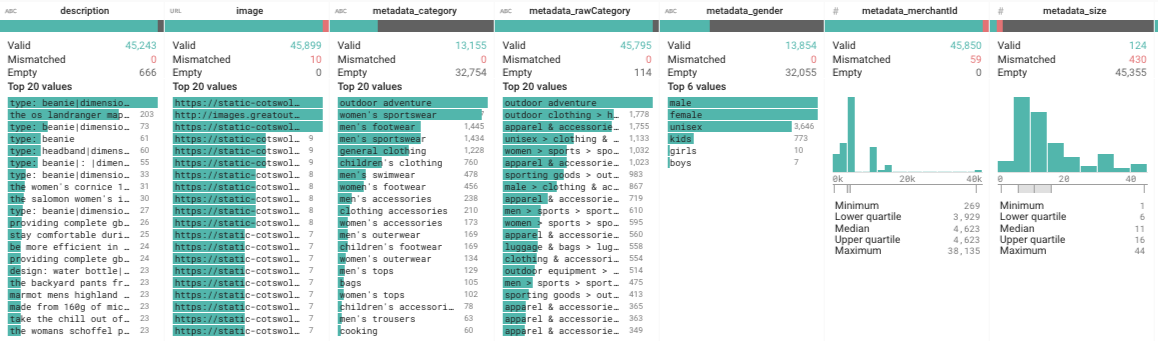
\includegraphics[width=1.4\textwidth]{figures/dataprep}
 \caption{Dataprep: the histograms of field values of a subset of fields.}
 \label{dataprep}
\end{figure}


The histograms revealed that a lot of the input features were mostly empty, but also that many of the inputs that would naturally be considered categorical  had much more unique value in them then one might expect.
For example, each affiliate gives us the textual representation what they consider to be the category of the product,  but  rather than containing a small number of unique tokens, these contained all the full category paths along with the category delimiters, which  varied retailer by retailer (e.g.  it was common to see both ``Shoes > Sneakers'' and ``Shoes // Sneakers'').
Representing these as categorical variables would have blown up the input space, which would have  resulted in more parameters, each parameter having fewer examples to learn from.
Therefore, many such ``categorical''  were actually represented as text, which were tokenised and cleaned appropriately, allowing for better generalisation and smaller models.

There was a single numerical field: price.
This could have been min-max normalised to the range 0 ... 1, however there  was a small number of very high values that would have squash nearly all the other  prices.
Rather than  carefully considering  how to mitigate this,  the input dimension was dropped, because it is not likely to have much predictive value for product classification.
It would be trivial to bring this feature back for a training objective for which it would be much more useful.

A trickier question was how many distinct tokens or categorical values to keep per input column.
Keeping all of them would not have been sensible: there were still large numbers of tokens that appeared only once, often because there were some unwanted formatting characters, misspellings, or incorrect punctuation that caused a token to be considered a separate entity.
There was a single configuration file that dictated which models used which features as input, whether those inputs were represented as textual, categorical, or dense values;  it also determined  the maximum number of unique values/tokens,  and the dimensionality of the embedding.
This configuration file was read by Dataflow during pre-processing  and by TensorFlow during  inference and training, which made experimentation with  different types of models and input representations considerably easier.

Below is a list of input features with information about how they were represented; it also lists the dimensionality of embeddings  for the models which  encoded categorical variables as embedding.

\begin{itemize}[noitemsep]
 \item title - text - max 8000 unique tokens
 \item brand - categorical - max 5000 unique values - 10 embedding dimensions
 \item category - categorical - max 950 unique values - 6 embedding dimensions
 \item rawCategory - text - max 1000 unique tokens
 \item description - text - max 8000 unique tokens
 \item gender - categorical - take all unique tokens
 \item size - categorical - max 100 unique tokens
 \item image - dense vector of 2048 or 1280 dimensions extracted with a 2D CNN
\end{itemize}


\section{System Architecture}
\label{architecture}

 The following technologies were used to build the system which had to interact with existing services  at the client company:

\begin{itemize}
  \item Apache Airflow (AF) - a Python framework for defining workflows of long-running tasks and dependencies between these tasks.
  \item TensorFlow (TF) - ML framework for Python, capable of defining many kinds of models as a computation graph, and executing this graph locally or in a distributed manner.
  \item ML Engine (MLE) - a GCP service for running TensorFlow models (training, hyperparameter tuning, inference).
  \item Apache Beam - a data processing engine akin akin to Apache Spark.
  \item Dataflow - a GCP service for executing Apache Beam workloads.
  \item Tensorflow Transform - a Python library with a small set of operations for data preprocessing that can run inside a TensorFlow graph as well as an Apache Beam pipeline.
  \item Google Cloud Storage (GCS) - Google Cloud Platform (GCP) object storage similar to Amazon S3.
  \item ElasticSearch (ES) - a NoSQL database with powerful full-text search and querying capabilities.
  \item RabbitMQ - a message queue, used for transferring data among our microservices (using the Logstash adapter, that can read from and write to (among other things) ElasticSearch and RabbitMQ).
  \item Flask - a simple backend web framework for Python.
  \item Node.js - a JavaScript backend web framework.
  \item React.js - a JavaScript front-end framework for JavaScript.
  \item Redux - a framework for persisting user interface (UI) state and application data in single page applications.
  \item GraphQL - a query language for building flexible APIs
\end{itemize}

Figure \ref{arch_diagram} shows the how data is passed between the main services, and how services and technologies interact.

All product data is stored in ElasticSearch (ES): the labels, top predictions of the ML system, and evaluation metrics from various train runs.
ES is accessed from the public web application via GraphQL and the ML administration web UI (further referred to just as web UI\footnote{The web UI was initially built with Flask and React by the author as a quick way to get insight about the model, and then re-written as a more feature-rich version by an employee of the client company with Node.js, GraphQL, React and Redux.}).
Data is pulled into the ML pipelines by dumping the results of an ES query to a local file, which is uploaded to GCS.
Updates to the ES index are not done directly, since indexing the updated products is computationally expensive; instead, updates are put on a RabbitMQ queue, which is consumed by Logstash, which in turn updates products in ES at a rate that will not overburden the servers.

All ML training and prediction happens in a batch-oriented way, encapsulated as Airflow pipelines.
Each pipeline is a directed acyclic graph of tasks, where a task can be a shell command or Python function; a pipeline defines dependencies of task execution, which allows us co-ordinate a series of operations that could be executed locally (inside the Docker container running AF) or remotely (such as in a GCP service).
A typical pipeline dumps data locally, uploads it to GCS, schedules a Dataflow job to preprocess data, polls the Dataflow service until the Dataflow job is finished, schedules an ML engine job, polls the MLE service until it has completed, and runs an update process that reads the predictions and evaluation statistics from GCS and sends the updates to the RabbitMQ queue.
Reading updates and sending these to RabbitMQ is done in a parallelised manner (using multiprocessing), since the update process is bottlenecked by network latency as well as computing the appropriate category path for each product (explained in \ref{cat_tree}).

\begin{figure}
  \hspace*{-0.2\textwidth}
  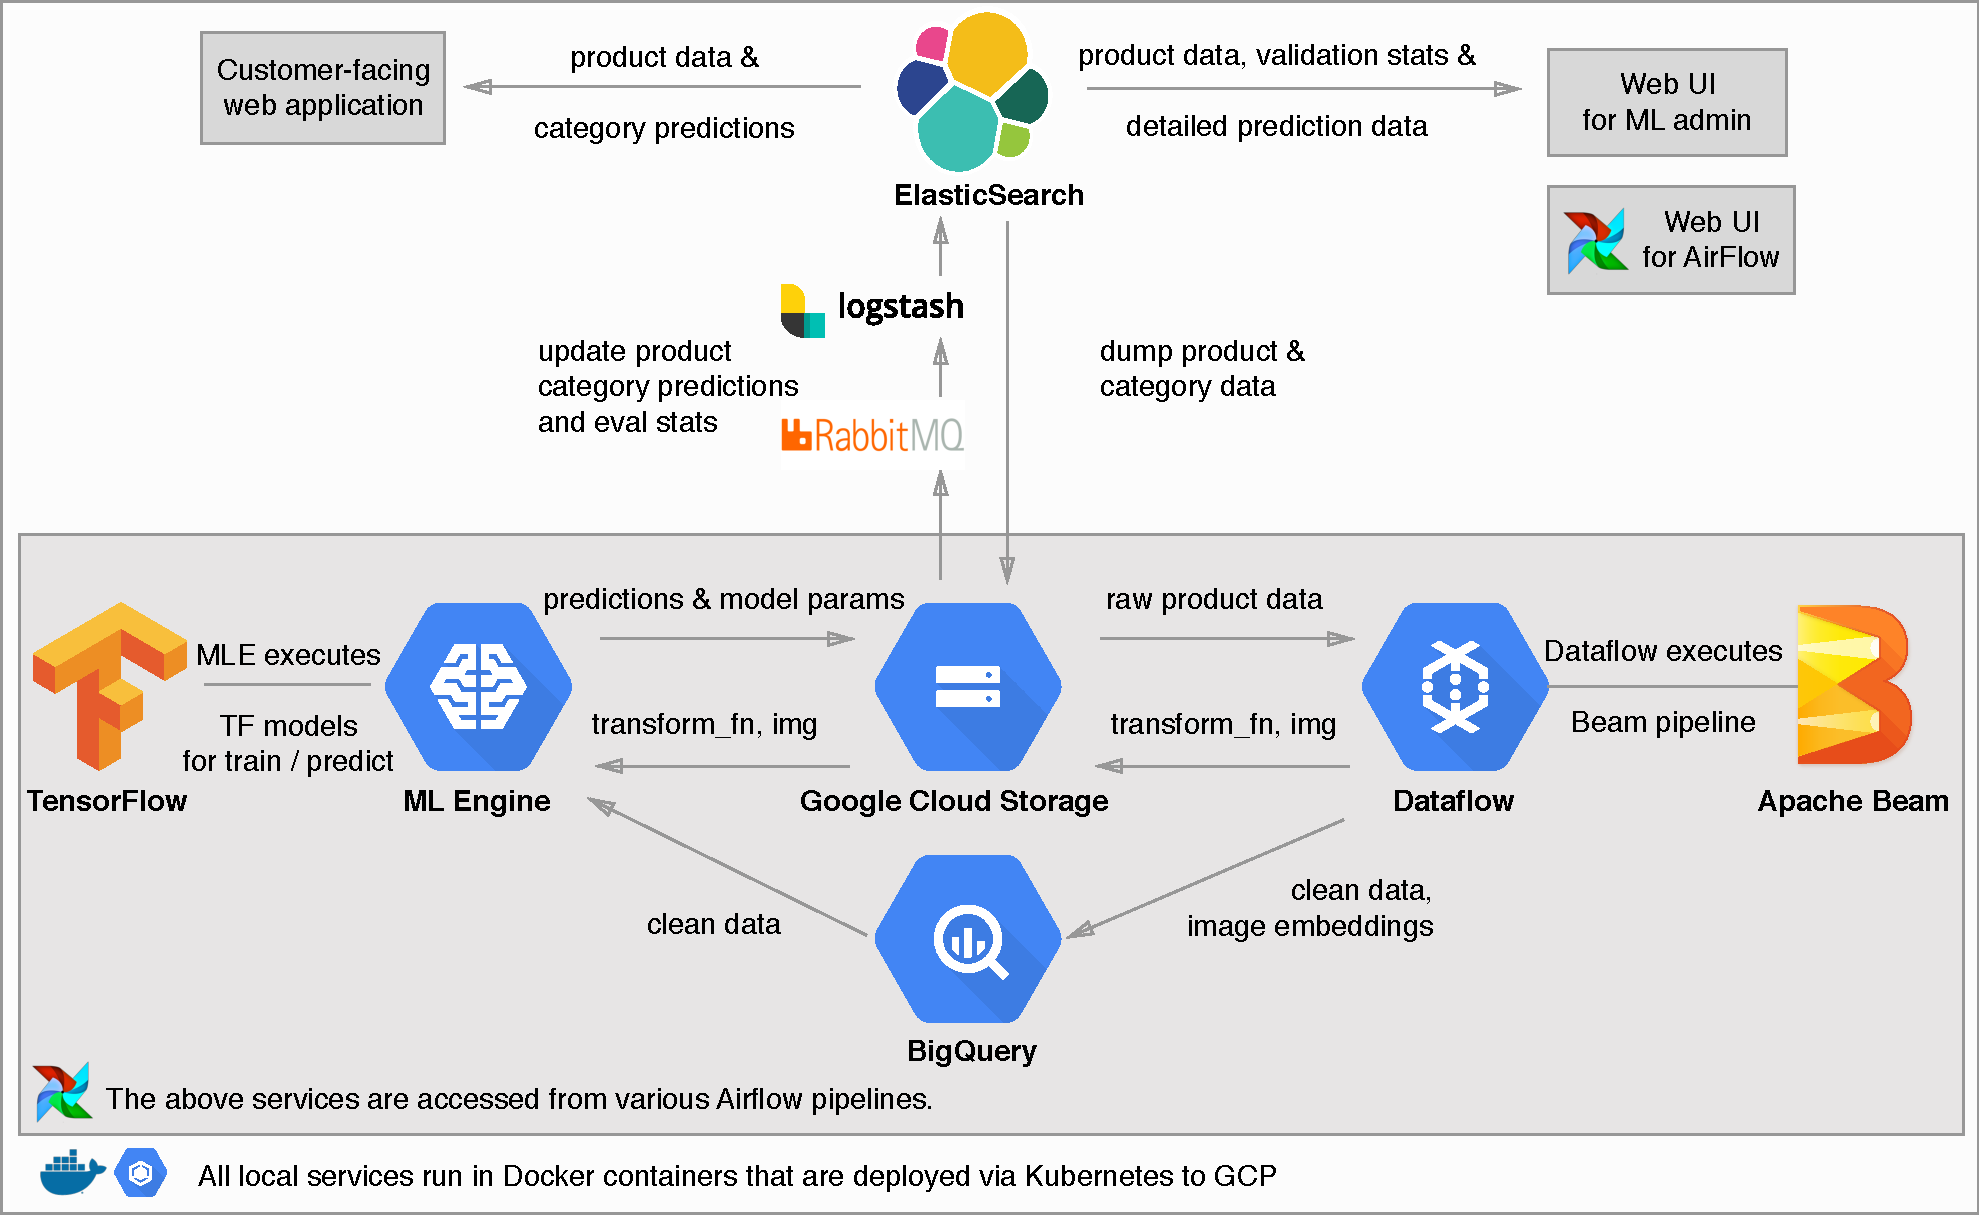
\includegraphics[width=1.4\textwidth]{diagrams/architecture}
  \caption{High-level system architecture of the ML pipeline}
  \label{arch_diagram}
\end{figure}

\subsection{Airflow Pipelines \& Pipeline Runs}

A group of tasks that would need to be run together repeatedly is encapsulated in an Airflow pipeline, which is a directed acyclic graph (DAG) of tasks (also referred to as an AF pipeline).
A DAG is run many times, either based on a schedule or triggered manually.
Figure \ref{fig:af1} shows a screenshot of the most common Airflow pipeline ``cat\_pp\_train\_specific'', which is short for ``categorisation: preprocess and train a specific model''; figure \ref{fig:af2} shows the sub-DAG of the task ``train''.

\begin{figure}
\centering
\begin{minipage}{.48\textwidth}
  \centering
  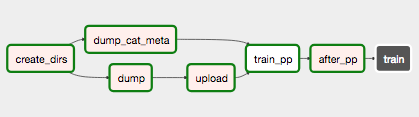
\includegraphics[width=1.0\linewidth]{figures/af_train_specific}
  \captionof{figure}{Airflow DAG: preprocess, train specific model, update statistics. All tasks except for ``train'' have completed, which is not yet scheduled for execution.}
  \label{fig:af1}
\end{minipage}%
\begin{minipage}{.48\textwidth}
  \centering
  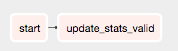
\includegraphics[width=.6\linewidth]{figures/af_train}
  \captionof{figure}{Airflow sub-DAG: train. No task has been scheduled for execution during this run.}
  \label{fig:af2}
\end{minipage}
\end{figure}

Most of our pipelines start by creating directories for our files.
Which files are stored where is configured in a simple file that is accessed by Airflow, Dataflow and TensorFlow (locally or inside MLE); the configuration has placeholders for variables that are determined per run or are specific to a task inside a run.
For example, the location of .tfrecords files is determined by ``\textit{:prefix}/runs/\textit{:run\_id}/ tfrecords/\textit{:objective}\_\textit{:split}.tfrecords'', where \textit{prefix} corresponds to the path to the data directory (either locally or in GCS), \textit{run\_id} is specific to the current run of the pipeline, \textit{objective} is either \textit{rule\_based} or \textit{exclusive}, and \textit{split} is either \textit{train}, \textit{test} or \textit{valid}.
This ensures that all parts of the system look for the same file in the same place, and makes building file paths easier.
All file access in the different parts work equally on a local file system and GCS, which makes it particularly convenient to switch between local experimentation and remote training; in fact, the \textit{prefix} parameter is by default read from an environment variable, which is different in local, Docker and cloud service environments.

A training dataset is identified by its \textit{run\_id}.
The processed .tfrecords, transform function (described below) and metadata is persisted under that run's directory.
Several models can be trained from the same dataset.
The checkpoints of a model are saved under ``\textit{:prefix}/runs/\textit{:run\_id}/checkpoints/\textit{:hparams\_id}/'', where \textit{hparams\_id} identifies a model architecture, as well as what kinds of training objectives and label types it is trained on; during hyperparameter tuning, a unique index is appended to the \textit{hparams\_id} of the model.
As \textit{hparams\_id} encodes only the general model architecture and training objectives, the full set of all hyperparameters is persisted along model checkpoints as a JSON file - for future reference.

\subsection{Dataflow Pipelines}
There are two types of Dataflow pipelines: for preprocessing training data and for calculating product-product visual similarity. Omitting various details, dead-ends and workarounds that were needed due to technical limitations and prior system architecture choices\footnote{which were completely reasonable at the time, when the ML system was not a consideration}, the pipelines had the following tasks:

\subsubsection{Preprocessing}
\label{pp}

This pipeline loads the products dumped from ES (as JSON) and preprocesses data according to a configuration file (see section \ref{data_pp}).
Figure \ref{df} shows a screenshot of this pipeline, as visualised by the GCP UI.

In this pipeline, all fields are cleaned of obvious noise and superfluous whitespace.
Text and categorical fields are tokenised and mapped to integer indices, keeping only the top \textit{k} values and also computing TF-IDF scores for text fields.
This is handled by TensorFlow Transform, which persists this token-to-index mapping in a \textbf{transform function} that is saved to GCS at the end of the pipeline.
The transform function can be used by TensorFlow or Dataflow to convert raw text inputs to a  sparse inputs;
separate pre-processing run will generate a different transform function, with mostly the same tokens mapping to different indices, as the order in which they will be encountered will be different.
The tokenised data is stored to GCS as a sharded .tfrecords files (with one set of files per training objective), a binary file format that TF Transform helps produce; alternatively the raw data could be saved (e.g. as JSON or inside BigQuery) and the transform function inside a TF graph could re-tokenise this raw data at runtime.

\begin{figure}
  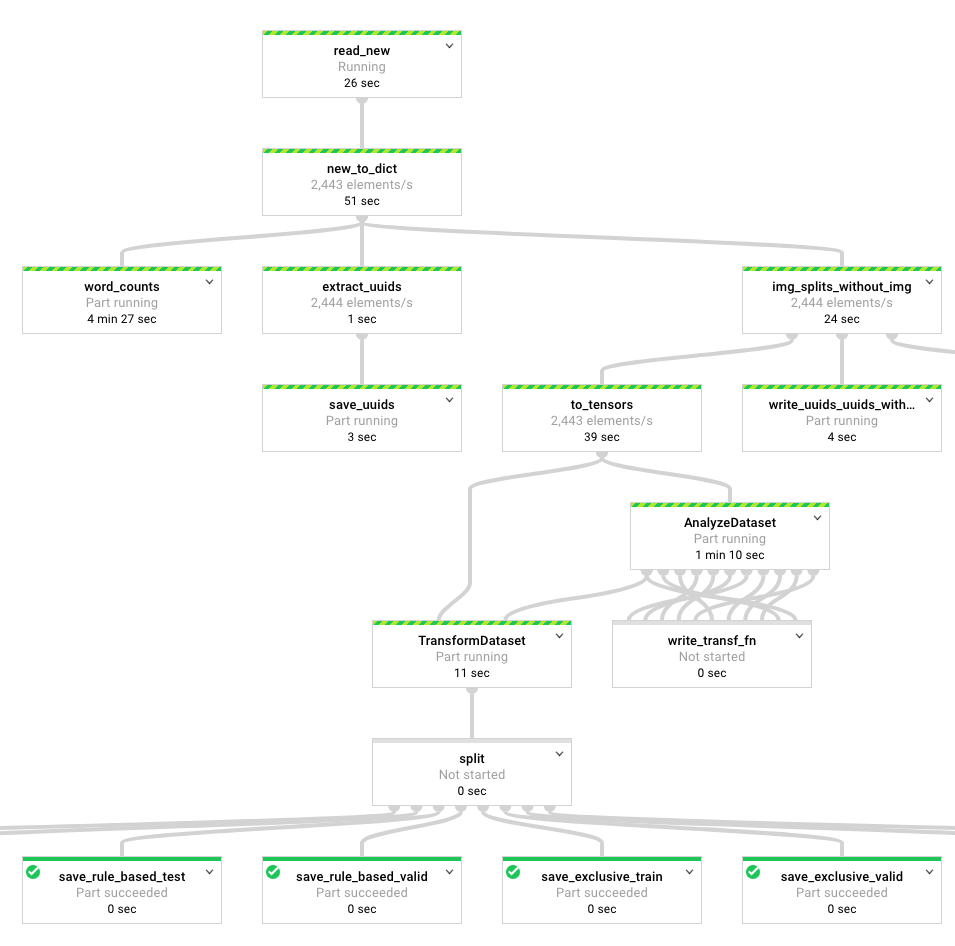
\includegraphics[width=\linewidth]{figures/df}
  \caption{A running Dataflow pipeline of data preprocessing}
  \label{df}
\end{figure}

The pipeline is also responsible for downloading product images, which are saved to GCS as individual files to avoid hitting the content delivery network that stores product images multiple times.
Images are a major bottleneck due to network latency.
To avoid a TF / MLE job from making separate requests to fetch each file individually\footnote{Each request has latency overhead, which compounds quickly when doing million of these.}, Dataflow saves the raw image content into the .tfrecords file; this increases Dataflow execution time, but reduces time and cost overall, as Dataflow is cheaper and easier to parallelise than a MLE job.

A former version of the pipeline also computed image embeddings inside the Dataflow job, but this was inefficient.
We also wanted to have the flexibility to try different models for computing embeddings (e.g. Inception V3, MobileNet, AutoML models) and fine-tuning image models.
Attempts to persist these pre-computed embeddings had severe overheads, and currently the approach is to re-compute these at every time inside MLE, which can leverage a GPU to do it efficiently.

\subsubsection{Visual Similarity}
\label{vis_sim_pp}

The Dataflow pipeline implemented for the experiments described in \ref{exp_sim} relied on image embeddings computed by the preprocessing pipeline.
As explained in section \ref{exp_sim}, it needs to find the \textit{k=100} nearest neighbours of each product based on the cosine similarity of their image embeddings.
The product-product  similarities are the simplest case computed within products that belong to same second level category.
The pipeline read the files output by the preprocessing stage, and partitioned it into datasets by the category predicted in the previous train run, as the new predictions would not be saved in the file.
The per-category image embeddings were merged (using \textit{reduce}) into matrices of image embeddings in a given category, and the top 100 approximate nearest neighbours were extracted for each product using nmslib \cite{nmslib} (as a \textit{map} operation over all the per-category embedding matrices).
The nearest neighbour UUIDs were persisted to GCS and a downstream AF task picked these up and updated ES with these.

This set-up will be replaced in the future.
Computing embeddings in Dataflow is slow, and me way want to enable more flexible ways of restricting the subset of products that are considered (e.g. not just 2nd level category, but a 3rd level category or even globally).
The most flexible approach is one in which nearest neighbours are computed in real time when a product is viewed by a user.
The biggest challenge in such a system is keeping all the image embeddings in memory, which would require 32 GB of memory for the 4 million products we currently have\footnote{$~4000000 * 2048 * 32$ = number of products * embedding dimensionality * 32 bits per number}, and the number of products is likely to increase in the future.

An option worth considering is deploying this as a TensorFlow model to MLE, which reads the embedding matrix in as a sharded tf.Variable; the shards can be distributed on different machines, which is handled automatically by TF.
The input to this model would be just the UUID of the product in question, and the UUID of the category to which the nearest neighbour search is limited; the ``prediction'' of the model would be dot product of the product embedding in question, and all the other product embeddings that are in the given category.
Therefore to get the nearest neighbours of an image embedding, TF would go through all the product embeddings to check for their membership of the given category - but this is fast given all the embeddings are always kept in memory.
The nearest neighbour search will also be precise, which would be prohibitively slow when pre-computing nearest neighbours but should be manageable when done online, as there will be only a handful of requests per second and the dot products are calculated in parallel by multiple workers.
We can also use autoscaling that would increase the number of workers to handle high loads, which would also put all workers to sleep after 15 minutes of inactivity.


\subsection{TensorFlow and ML Engine}

All models were implemented using TensorFlow, using higher level APIs (such as tf.data, tf.estimator and tf.learn) when possible.
This was somewhat challenging, as the high-level APIs were poorly documented, changed even throughout the duration of this project, and it was not clear which APIs are compatible with each other.
Ultimately the only reliable way to understand a class or function was to read its source code.
In many cases these APIs provided almost what was needed, but to support our use case the code was copied from the TensorFlow GitHub repository and adapted to our purpose\footnote{For example, multi-objective learning where each objective potentially changes a subset of the model's variables was not possible due to the way loss from multiple ``heads'' was merged in the current TF APIs. Also some parts had to be rewritten to give us per-class evaluation metrics.}.

The point of entry to the trainer program is the controller.py, which decides based on command line arguments which task to run: train, predict, train and predict, evaluate, export model, etc.
There is a large number of hyperparameters that can be supplied via command-line arguments, with reasonable defaults.

The data was loaded using the tf.data.Dataset API, which provide convenient functions for reading large numbers of files, prefetching, shuffling, batching, and performing arbitrary transformations on the data, such as transforming a set of bytes representing a JPEG image into a 3D tensor of integers.
This works well for simple use cases but is less flexible when for example doing multi-objective learning.
We would like to control roughly how many data points from each objective end up in a batch, or for how long a model is pre-trained on one objective before the second objective is introduced.
Refer to section \ref{multiobj} for a description of two approaches that were tried.
In general, the trainer program would use tf.data.Dataset class to build an \textit{input function} for either training or evaluating, and the input function would be supply data points for the train loop.

TensorFlow models were built using the tf.estimator.Estimator class by providing a custom \textit{model function}.
The model function would dynamically build the model based on the \textit{model type} (deep / linear), \textit{input type} (these are listed in section \ref{exp_models}), \textit{training objectives} and \textit{hyperparameters}.
An input type determines which input features are used and how they are represented, while a training objective determined which training dataset, loss function and evaluation metrics were used.
Both input types and training objectives had simple configuration files dictating their behaviour, which made adding new training objectives and experimenting with different model architectures easy.

Training was handled by the tf.estimator.train\_and\_evaluate function.
It loads a model from the checkpoint directory if present, and trains the model for a specified number of steps, or until the input function terminates.
It also periodically saves model checkpoints to GCS, and handles writing TF summary operations that are needed for data visualisations using TensorBoard\footnote{TensorBoard is a web interface for visualising the variables and metrics a TensorFlow train run produces; many of the visualisations in the following sections are taken from Tensorboard.}

\chapter{Method}
\label{meth}
\label{exp}


\hfill \break \noindent

Many kinds of experiments were conducted; the experiments, their evaluation and results are explained under the same subsection.
In section \ref{exp_sim} three visual similarity approaches are described and subjectively evaluated;
in section \ref{exp_models} we describe all the models that were trained to reproduce the behaviour of the rule-based system;
how multi-objective learning was used to improve the accuracy of individual training objectives is described in section \ref{multiobj};
finally, our efforts to reduce label complexity using active learning is described in section \ref{exp_al}.


\section{Visual Similarity}
\label{exp_sim}

Three approaches were tried for computing visual similarity.
In the first case, an approximate nearest neighbour method \cite{nmslib} was used on the image embeddings (as described in section \ref{vis_sim_pp}) and the top 100 predictions were saved to ElasticSearch.
In the second approach, the embedding vectors were discretised according to \cite{vec_fulltext} (as described in section \ref{bg_sim}) and inserted to ElasticSearch as strings of space-delimited tokens; standard ElasticSearch fulltext search was used on these token strings to get the nearest neighbour for a given product.
The third approach combined the similarity scores of the second approach and the original ElasticSearch title matching, as a single ElasticSearch query.

\subsection{Evaluation \& Results}

The evaluation of similarity scores is difficult, since it is inherently somewhat subjective.
A common approach is to hand-label triplets of images Q, A, B with four choices of how similar A and B are to Q.
These labeled triplets can be ranked using with similarity precision (percentage of triplets correctly ranked) and score at top K (see \cite{imgsimfineg}).
Creating this dataset of triplets would be a very time-consuming process. Therefore evaluation was done entirely subjectively.

Comparing the similarity between the former ElasticSearch title (ES title) matching and the new approximate nearest neighbour (ANN) search was straightforward - one look at the results was enough to confirm that the embedding-based approach outperforms title matching.
Figures \ref{shirt_es} and \ref{shirt_nmslib} show the nearest neighbours according to ES title and ANN, respectively; the image embeddings nicely pick up the pattern on the shirt, as well as the general style.
For some clothing categories this worked remarkably well, but with categories that had more varied products within it, there were occasional odd results.
For example, in the ``Hiking'' category, the nearest neighbours of sleeping bags could be items with seemingly similar shapes, such as a flashlight with a very zoomed-in product photo that had similar contours as an unrolled sleeping bag.
Another example of this is given in figure \ref{chair_nmslib}, which mostly returns chairs that are indeed visually and even functionally very similar to the chair in question - more so than the ElasticSearch title match seen in \ref{chair_es} - but also returns tables with similar legs; this is understandable, given that nearly half of the surface area of these images is covered by these foldable legs.
This problem can mostly be mitigated by having more fine-grained product categories and restricting the nearest neighbour search to those more specific categories.
The nearest neighbour similarity search may pick up qualities of the image that are not related to the product in question, such as background or fashion model; this is un-intended but is acceptable, and arguably creates a product listing which is more homogenous and therefore more aesthetically pleasing.

The second approach of discretised and tokenised image embeddings had mixed results.
The returned nearest neighbours were reasonable, but subjectively felt inferior to the ones computed from the raw image embeddings using ANN.
At times it felt like some aspect of the appearance dominated, which is understandable considering a lot of precision is lost when discretising the embeddings, and there is no theoretical justification why a TF-IDF score of these arbitrarily discretised tokens should behave similarly as a dot product between the original vectors.
With enough precision (using several discrete intervals per embedding dimension) this may well work, but this would incur a considerable performance overhead when indexing and querying.

The third approach of combining the existing title matching and discretised and tokenised vectors was somewhat successful.
As seen in figure \ref{chair_tokenised}, the title matching ensures that top results are at least about the same kind of items (chairs) while the tokenised embedding query returns products that share some visual similarity (mostly the legs of the chair).
This approach still suffered from similar problems as the second approach - poor performance and somewhat inconsistent visual similarity - while introducing an additional complication of finding a good weighting between the title and visual scores.
Given that there was no efficient way to evaluate the different weightings, it was decided to use raw image embeddings for visual similarity, either as an ANN search or a precise realtime version.

\begin{figure}
  \centering
  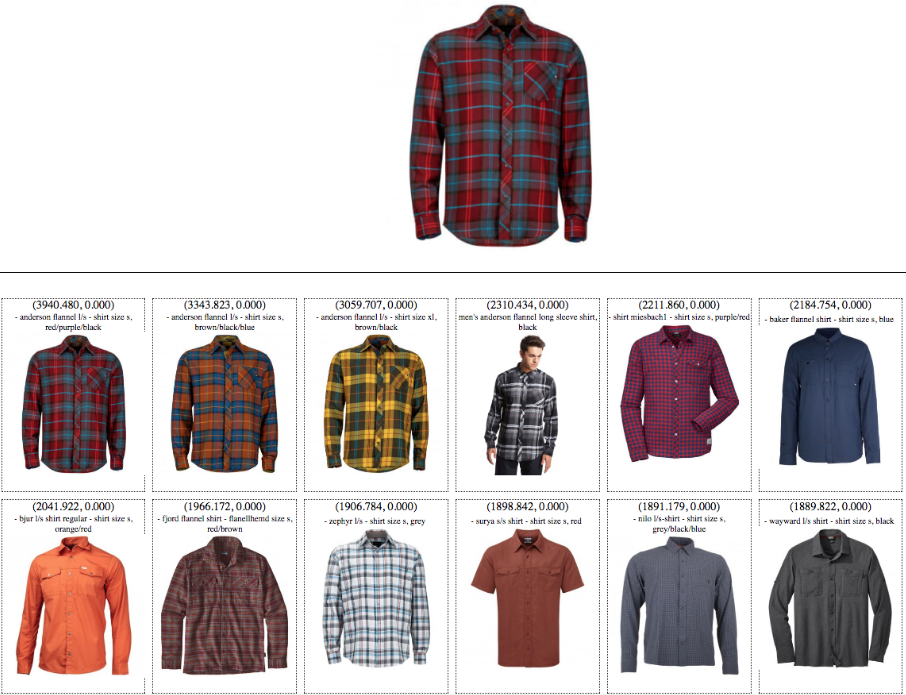
\includegraphics[width=0.8\linewidth]{figures/compare/shirt_es}
  \caption{Nearest neighbours based on ElasticSearch title matching (TF-IDF-like)}
  \label{shirt_es}
\end{figure}
\begin{figure}
  \centering
  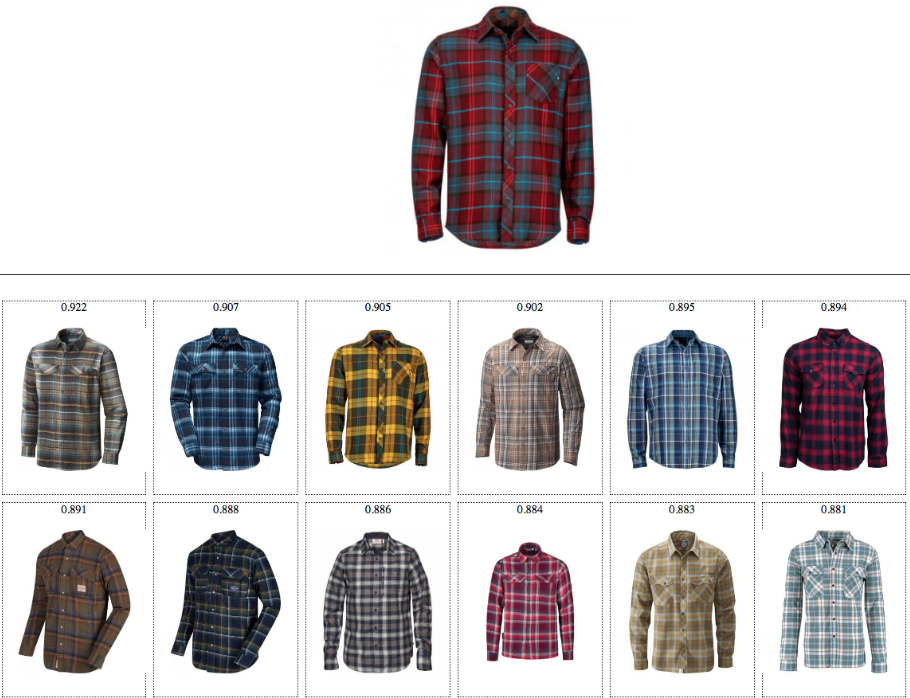
\includegraphics[width=0.8\linewidth]{figures/compare/shirt_nmslib}
  \caption{Nearest neighbours based on ANN search of image embeddings}
  \label{shirt_nmslib}
\end{figure}

\begin{figure}
  \centering
  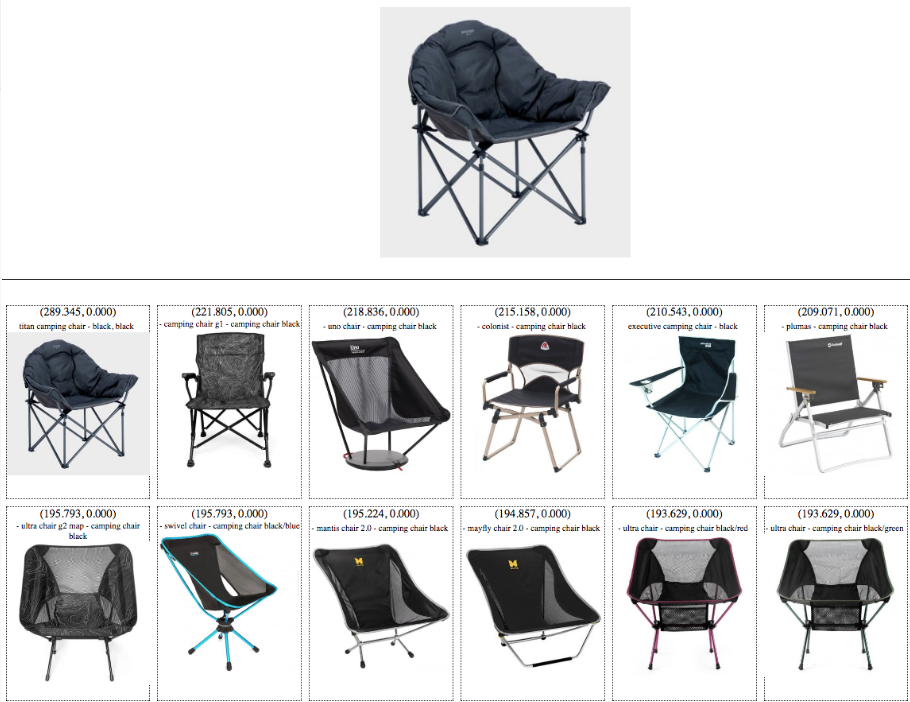
\includegraphics[width=0.8\linewidth]{figures/compare/chair_es}
  \caption{Nearest neighbours based on ElasticSearch title matching (TF-IDF-like)}
  \label{chair_es}
\end{figure}
\begin{figure}
  \centering
  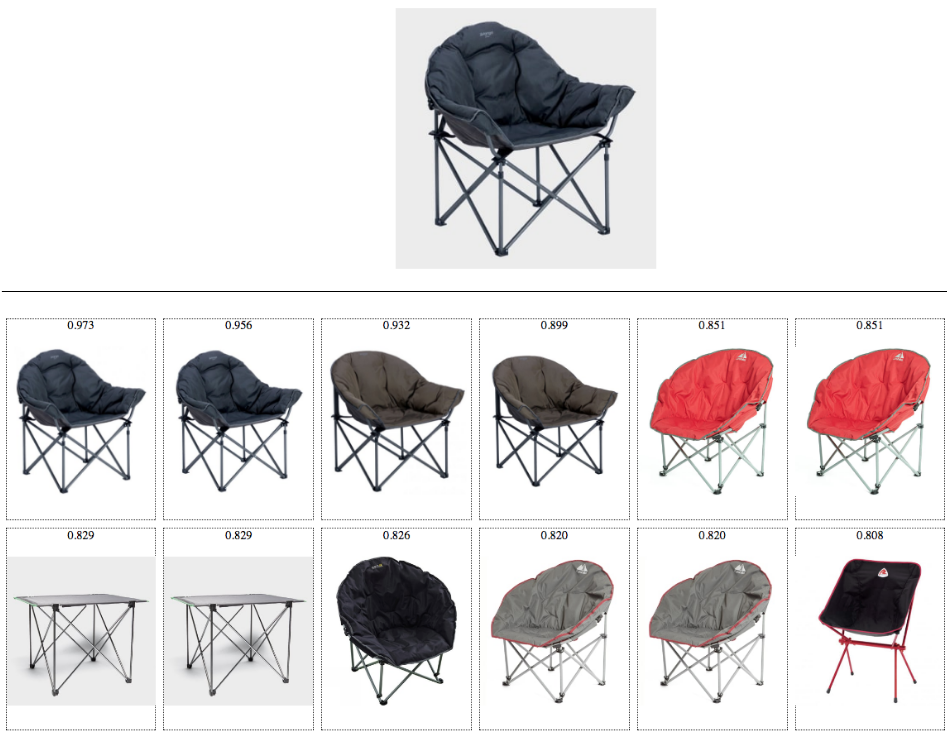
\includegraphics[width=0.8\linewidth]{figures/compare/chair_nmslib}
  \caption{Nearest neighbours based on ANN search of image embeddings}
  \label{chair_nmslib}
\end{figure}
\begin{figure}
  \centering
  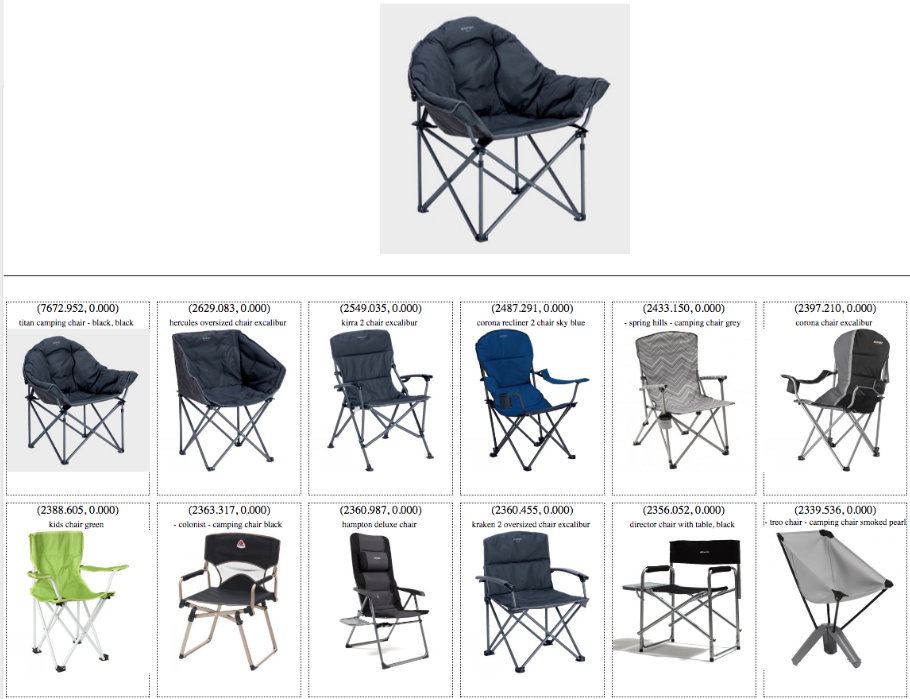
\includegraphics[width=0.8\linewidth]{figures/compare/chair_tokenised}
  \caption{Nearest neighbours based on fulltext search on discretised/tokenised image embeddings as in \cite{vec_fulltext}. Here scores from the title and image embedding fields was combined.}
  \label{chair_tokenised}
\end{figure}

\section{Independent Models}
\label{exp_models}

Several models were trained on the rule-based labels to find out which models can best replicate its behaviour.
We first describe the Wide \& Deep model that was trained as a baseline.
Then the different input features and how these were represented are described, along with how linear and deep models were trained from these input representations.

\subsection{Baseline Model: Wide \& Deep}
\label{widedeep}

As described in section \ref{bg_wide_deep}, the ``Wide \& Deep'' model consists of two models that are trained jointly using stochastic gradient descent: a deep and a shallow neural network which both predict the same set of binary outputs.
The original idea of Wide \& Deep was to use the wide component for feature crosses (e.g. of two categorical values), but in our experiments the wide component received mostly just the 1-hot encoded categorical inputs while the wide component received the same inputs as random embeddings (or as pre-computed image embeddings extracted with Inception V3 that is pre-trained on ImageNet).

Initial experiments with this model were done on a dataset of roughly 800 000 products which were labeled by the rule-based system\footnote{The database in the client company was in constant flux, so the training set sizes depended on how many labels the rule based-system had assigned to the current database. Still, when comparing different model architectures, we used a ``frozen'' version of the data to avoid skewing the results.}.
The data was partitioned into a train (\textasciitilde80\%), validation (\textasciitilde10\%) and test (\textasciitilde10\%) sets in the Dataflow preprocessing pipeline based on a pseudorandom number generator - assign the product in question to the dataset if the random number is in the range 0 ... 0.8, 0.8 ... 0.9, 0.9 ... 1.
The train set was used to train the model, and the validation set was used to evaluate the model periodically as it was trained - during individual training runs and during hyperparameter tuning.
The test set was held out for evaluating the model after hyperparameter tuning, but was not used due to the low variance in validation set error during the different tuning rounds.

\subsection{Input Representation \& Model Type Combinations}
\label{model_comb}

To assess which features are most useful for learning the rule-based objective, different features were grouped into \textit{input types}, shown in table \ref{input_types}.
The columns represent the input feature; refer to section \ref{data_pp} for the full feature names and their description.
Entries in the table show how each input feature was represented: \textit{emb} for for categorical features that are represented as random embedding vectors (which are updated during SGD), \textit{emb avg} for multi-token fields where tokens are represented as random embeddings and the input feature is a weighted sum of these embeddings\footnote{Each embedding vector is weighted by the number of times it appears in the input feature, and divided by the L2 norm of the token counts; this gives good results for bag-of-words inputs according to TensorFlow documentation:
\newline
https://www.tensorflow.org/api\_docs/python/tf/feature\_column/embedding\_column}.
Feature columns marked with \textit{u.s.enc} have been converted from raw text into dense embedding vectors of size 512 using a pre-trained model Universal Sentence Encoder \cite{uni_sent_enc}; cells marked with \textit{mobilenet} and \textit{inceptionv3} have respectively extracted image embeddings of size 1280 and 2048 using the Mobilenet \cite{mobilenet} and InceptionV3 \cite{inceptionv3} models that were pre-trained on the ImageNet challenge; these embedding models were used via TensorFlow Hub\footnote{TensorFlow Hub is a collection of TensorFlow models that are pre-trained on some other task and can be used as a feature extractor or as an initialisation for a model that is fine-tuned: https://www.tensorflow.org/hub/}.
Pre-trained models were used only as feature extractors, i.e. were not fine-tuned on our data.

\begin{figure}
  \centering
  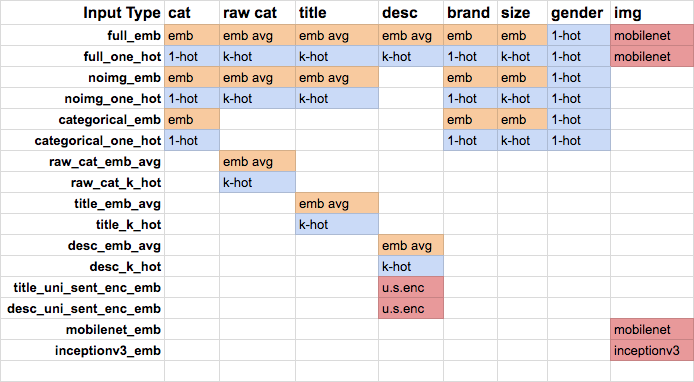
\includegraphics[width=\linewidth]{figures/input_types}
  \caption{Input types. Orange: embedding representation, blue: 1-hot or k-hot, red: embedding extracted with a pretrained deep network.}
  \label{input_types}
\end{figure}

Two model types were used to train with each of these 16 input types: linear and deep.
Like in the case of the baseline model, the \textasciitilde1.2 million data points were split into train/validation/test sets (80\%/10\%/10\%); train and validation sets were used during individual training runs and hyperparameter tuning.
All 32 combinations of input and model type were trained using hyperparameters listed in table \ref{tuning_rounds} column \textit{Deep (rb all)}.


\subsection{Evaluation}

Many metrics can be used to evaluate \textbf{multi-label classification}:

\begin{itemize}
  \item TP, TN, FP, FN: true positives, true negatives, false positives, false negatives,
  \item accuracy: $\frac{TP + TN}{FP + FN}$, fraction of correct predictions,
  \item precision: $\frac{TP}{TP + FP}$, fraction of positive predictions that were correct,
  \item recall: $\frac{TP}{TP + FN}$, fraction of positive labels that were correctly ``recalled'',
  \item F1: $2\frac{precision * recall}{precision + recall}$, harmonic average of precision and recall,
  \item TPR = recall: $\frac{TP}{TP+FN}$, true positive rate, probability of detection,
  \item FPR: $\frac{FP}{FP+TN}$, false positive rate, probability of false alarm,
  \item ROC AUC: the area under the curve of TPR plotted against FPR.
  \item PR AUC: the area under the curve of precision plotted against recall.
\end{itemize}

In our case, an overwhelming number of labels are negative, therefore a very simple predictor (that predict ``negative'' for every product / category) would have an accuracy near 99\%; ROC AUC is not suitable for the same reason, as a big change in FPs would result in a small change in FPR due to large TNs squashing FPR to a small number (see \cite{prauc} for details).
Precision and recall are useful measures to understand the model: it is expected to see a sharp increase of precision and decrease of recall as the model learns to predict ``negative'' for most classes, followed by a gradual increase of recall as the model learns to predict ``positive'' for the correct classes.
Precision and recall are competing metrics: increased precision tends to lead to decreased recall and vice versa, therefore models which combine the two are suitable for evaluating multi-label prediction problems with unbalanced classes.
While F1 score gives the harmonic mean of precision and recall at a given threshold, PR AUC paints a more complete picture by showing what the ratio would be at all the threshold values\footnote{There are infinitely many threshold values in the range 0 ... 1, so naturally we consider a small number of threshold values when approximating AUC.}.
Therefore, all evaluation of multi-label classification is based on PR AUC, i.e. when choosing between model architectures or hyperparameters, a model with a higher PR AUC is preferred.
Refer to \cite{prauc} for an explanation why PR AUC should be a preferred metric for highly imbalanced binary classification problems.

\subsection{Results}


\paragraph{Wide \& Deep}
The PR AUC on the 800,000-item dataset for this model after hyperparameter tuning was 0.9981 (see section \ref{tuning} for a full description of the set-up).
A manual examination of the predictions revealed that the top predictions for most categories was high-quality, but there was a large number of products below the decision boundary that actually belonged above it.
A later run of the model on 1.2M products gave an PR AUC of 0.8647; this was using the hyperparameters that the tuning step produced, so it is likely that the decreased AUC PR score is caused by a bug\footnote{Two explanations seem most likely: (1) the initial PR AUC was artificially high as some of the test set products ended up in the training set; (2) when migrating from the 800k dataset to the 1.2M dataset, the image embeddings were transferred over as an attempted optimisation approach, which may have mixed up image embeddings between products.}.
There were occasional odd results from the model once it was trained on the 1.2M dataset; it was hard to tell which part of the model was causing it, or even whether all the input features are actually improving predictive power; therefore, a more systematic approach was tried, explained in the next section.

\paragraph{Input Representation \& Model Type Combinations}

Table \ref{metrics_all} shows the precise PR AUC and recall scores of the final time steps.
The training loss function of linear and deep versions of noimg\_emb is shown in figure \ref{train_loss_all}.
The PR AUC on the validation set is shown in figure \ref{pr_auc_all}, where each model is trained for 300 000 batches, which is roughly 6 epochs; similarly, figure \ref{recall_all} shows how recall changes during the course of training.
The PR AUC on the final step (300k, or 220k for inceptionv3) is shown in figure \ref{pr_auc_chart}; recall plot of the final time step was omitted, as it was very similar to the final PR AUC scores.

\begin{figure}
  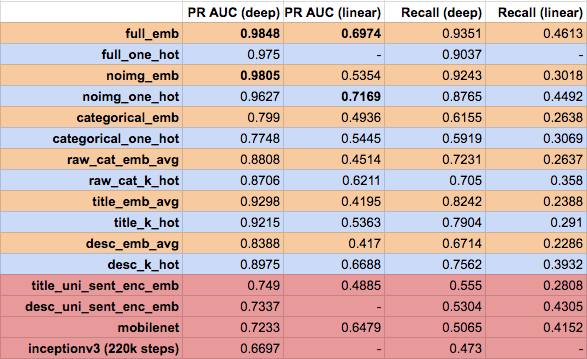
\includegraphics[width=\linewidth]{figures/metrics_all}
  \caption{Evaluation metrics of the rule-based training objective on the final time step. Minus denotes a train run that was not scheduled (inadvertently).}
  \label{metrics_all}
\end{figure}

\begin{figure}
  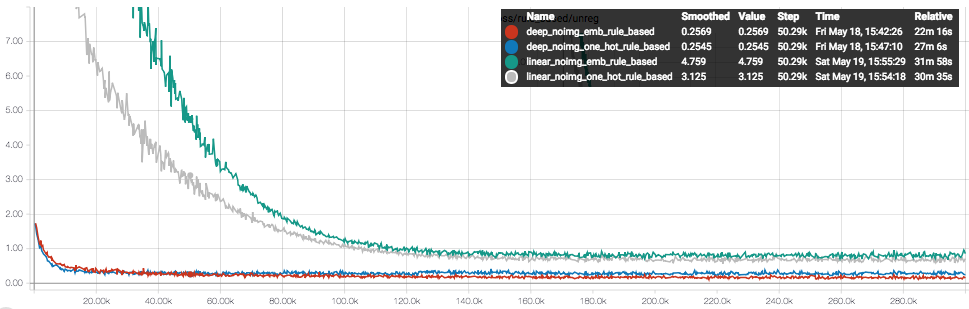
\includegraphics[width=\linewidth]{figures/train_loss_all}
  \caption{x axis = train step (batch number), y axis = training loss of rule-based objective.}
  \label{train_loss_all}
\end{figure}

\begin{figure}
  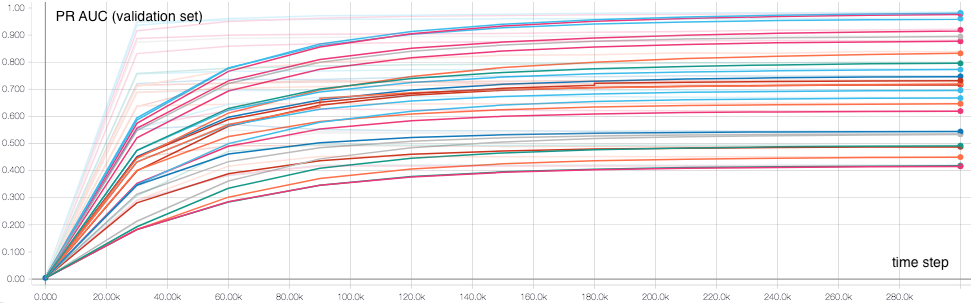
\includegraphics[width=\linewidth]{figures/pr_auc_all}
  \caption{PR AUC of all combinations of input and model types; x axis = train step (batch number), y axis = PR AUC. Refer to figure ... for exact scores.}
  \label{pr_auc_all}
\end{figure}
\begin{figure}
  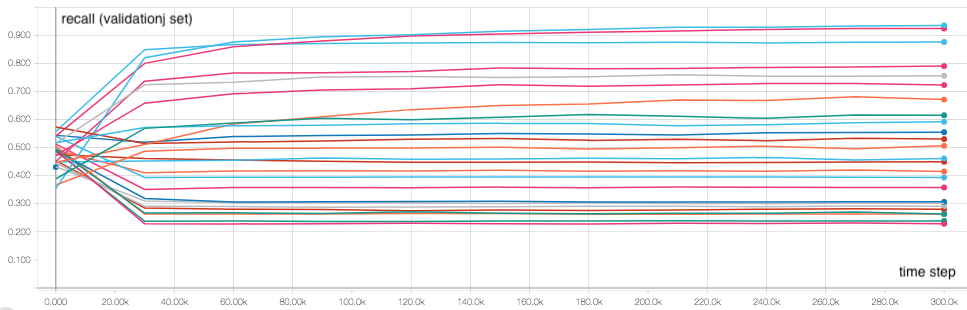
\includegraphics[width=\linewidth]{figures/recall_all}
  \caption{Recall of all combinations of input and model types; x axis = train step (batch number), y axis = recall..}
  \label{recall_all}
\end{figure}

\begin{figure}
  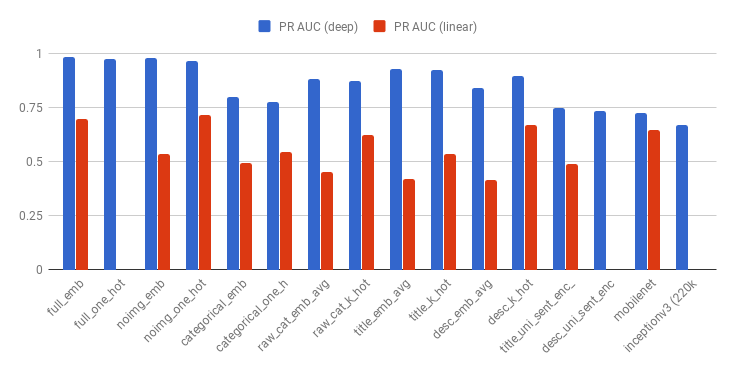
\includegraphics[width=\linewidth]{figures/pr_auc_chart}
  \caption{PR AUC on final timestep (300k, or 220k for inceptionv3)}
  \label{pr_auc_chart}
\end{figure}


\section{Multi-Objective Training}
\label{multiobj}


\subsection{Category Structure}
\label{cat_tree}

At the time of writing, there were roughly 1300 categories defined in the client database.
Categories were structured in a way that is typical of  e-commerce:  categories can have  child categories, which in turn can have child categories, etc.

Categories can be considered as independent (multi-label, sigmoid activation) or mutually exclusive (multi-class, softmax output layer); the difference is shown on a Venn diagram in figure \ref{excl_ind}.
The common way to handle this is to assume categories are mutually exclusive.
With exclusive categories, assigning a label to a product determines its label across all categories, whereas with independent categories a positive label only determines the label regarding the category in question (and its ancestors in the category tree) - that is roughly a thousand-fold difference in labelling efficiency.
The prediction task is also easier for exclusive classes - rather than needing to predict a probability score above a threshold separately for each class, the model would need to just assign the highest probability to the correct class compared to other classes.
On the other hand, some categories at the client company are inherently ambiguous or even overlapping.
The rule-based labels are also independent, since a product may be labelled to belong to zero or many categories.

\begin{figure}
  \centering
  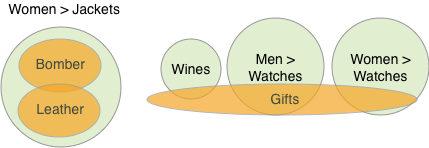
\includegraphics[width=0.6\linewidth]{figures/slides/excl_ind}
  \caption{Exclusive (green) vs independent (yellow) categories. A product belonging to a mutually exclusive category would not belong to any other category (e.g. a jacket is never a wine), while a product can belong to many independent categories (e.g. the same jacket can be a bomber jacket as well as a leather jacket). }
  \label{excl_ind}
\end{figure}

Bearing in mind the considerable efficiency gain in labelling, we mark a subset of the categories (1063) as ``exclusive''.
Exclusive categories are usually leaves, but at times a higher-level category was marked as exclusive, denoting the more general case\footnote{e.g. if ``Books'', ``Books > Travel Books'' and ``Books > Cookbooks'' are all marked as exclusive, then the semantics of ``Books'' is actually ``Books that are not about travel or cooking''. This means some categories are not strictly exclusive, but we had to work around the existing category structure.}.
Therefore we have \textbf{two training objectives}: a multi-label prediction of independent categories labelled by the rule-based system, and a multi-class prediction of exclusive categories labelled by the employees of the client company - respectively called the \textbf{rule-based} and \textbf{exclusive} training objectives.

We can not use the rule-based labels directly for training the exclusive objective; even if they share the same set of categories, the logits (the value before the softmax/sigmoid activation) of multi-class and multi-label classification behave differently, so we can not just copy the parameters learned from rule-based objective to the exclusive objective.
We can either do multi-objective training where the neural network has two output layers: one for the exclusive and one for rule-based objective (see figure \ref{multiobj_model} for a depiction of this multi-objective model).
Alternatively, we could convert the labels assigned by the rule-based system (which are inherently independent) into exclusive labels; we call this training objective \textbf{``exclusivised''\footnote{This word does not exist in dictionaries, but its meaning should be clear.}}.
This would allow us to train with only a single training objective, where most labels are assigned using the rule-based system and ``exclusivised'', and a small number of labels comes from human labellers; this approach might have benefits as the output layer would receive far more examples compared to the exclusive objective in the multi-objective training scenario.
To do that, we look at all the rule-based labels of a product that are applied to categories marked as exclusive.
If there is only one such label assigned, as would be for most products, the label is already exclusive; if there are more than one such label, we can either insert the product to the training set twice (once for each label), or select a random label.
We chose the latter approach.


\begin{figure}
  \hspace{-20pt}
\begin{subfigure}{.5\textwidth}
  \centering
  \includegraphics[width=\linewidth]{figures/slides/multi_objective_model_RB}
\end{subfigure}%
\hspace{20pt}
\begin{subfigure}{.5\textwidth}
  \centering
  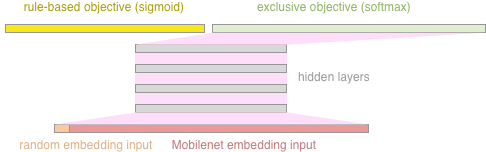
\includegraphics[width=\linewidth]{figures/slides/multi_objective_model_ex}
\end{subfigure}
\caption{A multi-objective model. Left: gradients (pink) when a rule-based label is present. Right: gradients (pink) when an exclusive label is present.}
\label{multiobj_model}
\end{figure}

% \label{label_imbalance}
% The labels provided by the rule-based system are only positive:  some products are labelled to belong to a given category, but many products that ought to belong to a category are not labelled  accordingly -  but their label still appears to be negative.
% This (which we call the \textbf{label imbalance} problem) only exacerbates the \textbf{class imbalance} problem (that most products do not belong to most categories).
% As a result the model trained on rule-based labels will certainly underestimate the likelihood of any product belonging to any category.


\subsection{Labelling of Exclusive Products}
\label{labex}

There were three purposes for labelling products: (1) creating a validation set, (2) creating an initial dataset for training the exclusive outputs so that reasonable uncertainty scores could be computed for active learning, and (3) labelling during active labelling rounds.
There are three ways of picking products to be labelled: random sampling (a product is sampled randomly from all products that do not have an exclusive label), uncertainty sampling (the unlabelled product with the highest prediction entropy is chosen), and searching for a product manually using our web UI.
When saving a label, the relevant metadata about how the product was sampled is also persisted to enable filtering out certain types of labels when running experiments.

In the experiments of the following section, the validation set contained 509 randomly sampled products and 5439 products that were manually searched for; for training set the equivalent numbers were 509 and 5646.
Initially random sampling was used to obtain labels for products, to avoid bias in gathering data only through title search.
Yet this approach would have taken a long time to populate all categories in the validation set with products, therefore the labelling team went through each existing category one by one and added ~5 products to the test and validation set using title matching.

% Each of the three datasets is represented by a separate set of tfrecords files; these were produced by Dataflow during the preprocessing stage described in section \ref{pp}.
% Each objective had two sets of files that corresponded to the training and validation datasets.
% For the rule-based objective, this was done based on random splitting; for the exclusive objective, this was done based on a boolean variable the human labeller could specify (``assign this product I am labelling to the train or validation set'').
% The exclusivised validation set had the same products as the exclusive validation set, and the exclusivised train set contained all the ``exclusivised'' rule-based labels as well as all the labels from the exclusive train set; when both an exclusivised and manual exclusive label were available, the latter was used.
% The train and test set sizes were as follows: rule-based (1.14M / 142K), exclusive (6K, 6.6K), exclusivised (1.24K, 6.6K).

\subsection{Evaluation}


As described in section \ref{cat_tree} we have three distinct training objectives: \textit{rule-based}, \textit{exclusive}, and a hybrid \textit{exclusivised}.
The models described in the previous section were trained only on the rule-based objective.
In this section we see how a performant models from the previous section performs when trained on the exclusive objective (from a small number of hand-assigned labels), how jointly training using both the rule-based and exclusive objective improves the accuracy of the exclusive objective, and how it compares to the ``exclusivised'' training objective.

For the exclusive objective, which is an instance of \textbf{multi-class classification}, accuracy is a reasonable measure.
Even though classes are imbalanced (``Dresses'' has more products than ``Travel Books''), there is no single dominant class that could be used as a shortcut by the model.
On the other hand, similar problems arise with evaluating multi-class problems where there is potentially overlap between some classes: the metric would give a low score even if the model predicted a semantically very similar class, or a more general class instead of the more specific one it was labelled as.
Therefore a manual evaluation of the misclassified products is needed to determine whether the error rate is caused by the ambiguity of the classes or by problems with learning.

\subsection{Experiments \& Results}

\subsubsection{Combining Data From Objectives}

To train jointly for the rule-based and exclusive objectives, the data from the different datasets had to be combined.
In the naive version, data from both datasets is loaded into memory and shuffled, but this would not work when we are also loading images or the dataset size grows.
As a scaleable workaround, we read the file names of each objective into memory (a few hundred to a few thousand in our case), shuffle the file names, and alternate between reading $m$ files from the first objective and $n$ files from the second objective (we used $m = n = 1$); when one dataset runs out of files, wrap around, but if the other objective also runs out of files, terminate producing filenames.
The resulting stream of filenames is read by a tf.data.Dataset, which loops through the produced filenames indefinitely and keeps a shuffle buffer of $b$ elements; within this buffer the data points from the different objectives get mixed up, so each training batch usually gets products from both objectives.
Note that the file shards are of different sizes: how many products end up in each file depends on how many Dataflow workers were used and how load was divided among those workers.
Therefore, to avoid long periods where batches are filled with data points from a single objective, larger shuffle buffer sizes should be used.

Another simple option for combining data from different objectives is to dump all data in the same file, and optimise the model's parameters with respect to all the objectives for which your items in the given batch have labels for.
This ensures that data points are seen an equal number of times, but is problematic when the different objectives have vastly different number of labels, as there is no good way to force training on the under-represented objective more heavily.
An additional unforeseen problem occurred with this set-up: due to the way data was pre-processed, the data points from the exclusive objective often ended up in a single file, which resulted in terribly unstable training unless the shuffle buffer was the size of the whole dataset.
This can be seen in figure \ref{pretrain}, where the training loss of the rule-based objective (magenta) shoots through the roof once it encounters its first exclusive data point.
In this case it happened a late stage, when the model had trained for nearly 4 epochs' worth of data\footnote{Due to the way the input function that feeds data to the model is restarted every time the model is evaluated, there is no guarantee that all files/data points are accessed the same number of times. So it is possible the chunk with all the exclusive labels comes at a late stage or several times.}, and by that time the adaptive learning rate of Adam has already learned that the weights of the exclusive output layer are never updated, i.e. the next update should have a very strong learning rate.
Now when the model sees all the exclusive labels at once, the gradients are big enough to affect the whole network, which is why the changes are visible even in the loss function of the rule-based objective; many other metrics (such as L2 regularisation loss and gradient norm) also grew sharply at the time step when exclusive and rule-based losses blew up.

\subsubsection{Pretraining on the Rule-Based Objective}

The initial plan was to pre-train the model on the rule-based objective, and then train jointly on both objectives.
As seen on figure \ref{pretrain}, the training loss of the rule-based objective (blue) makes large periodical jumps, followed by periods of high-variance downwards fluctuation.
The first such jump starts after the first epoch of pre-training, and following jumps can leave the loss function plateaued on the level it jumped to.
The sharp jumps can be explained by the high learning rate set for the parameters of the exclusive output layer that have received few or no updates, and the subsequent plateau of the loss function could be explained by the fact that the learning rate for the rest of the model has been reduced substantially, and the model (which is shaken up from its position near an optimum) is unable to escape its new sub-optimal ``valley'' of the loss surface.
Contrast this with figure \ref{nopretrain}, where the jointly trained model's loss (red) is gradually converging towards the loss of the single-objective loss (blue).
In figure \ref{pretrain} all the other parameters are the same as in \ref{nopretrain}; the former uses pre-training and the latter does not, and obviously the runs had different outcomes when shuffling data.

\begin{figure}
  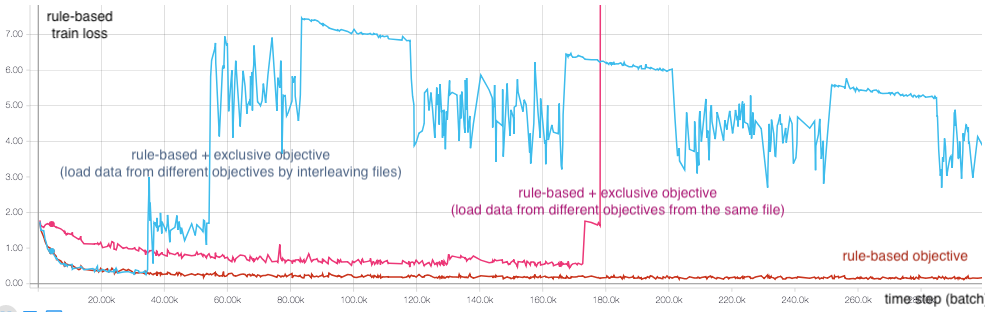
\includegraphics[width=\linewidth]{figures/multiobj/pretrain}
  \caption{Unregularised training loss of rule-based objective. Red: only rule-based objective. Blue: until step 35K, only rule-based objective, then a combination of rule-based and exclusive. Magenta: rule-based and exclusive objectives loaded from the same files. Shuffle buffer size: 15K.}
  \label{pretrain}
\end{figure}

\begin{figure}
  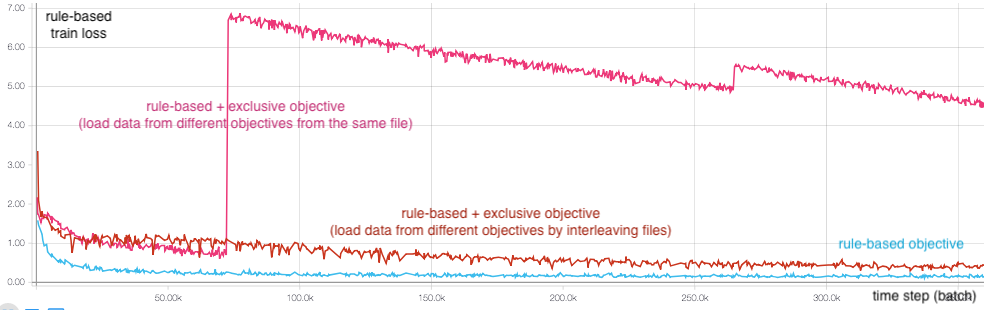
\includegraphics[width=\linewidth]{figures/multiobj/nopretrain}
  \caption{Unregularised training loss of rule-based objective. Blue: only rule-based objective. Red: combination of rule-based and exclusive objective. Magenta: rule-based and exclusive objectives loaded from the same files. Shuffle buffer size: 15K.}
  \label{nopretrain}
\end{figure}

\subsubsection{Exclusive, Exclusive \& Rule-Based, and Exclusivised Objectives}

Our real goal is to properly predict the exclusive objective.
As is evident from figure \ref{ex_vs_joint}, the model trained with just the exclusive objective converges fast and improves little after the first epoch, while the stable multi-objective model continues to improve in accuracy after several epochs, surpassing the single-objective accuracy after about three epochs.
The PR AUC of a model trained on just the rule-based objective exceeds that of the multi-objective training, which can be explained by the additional variance the exclusive objective introduces.
Both results are as expected, though the overall accuracy of 60\% is not particularly strong.
A reasonable guess is that the parameters of the exclusive output layer did not receive enough training examples to learn from, so a model was trained on the exclusivised data set as well.
Alas, as seen in figure \ref{ex_vs_exclusivised}, the exclusivised training objective does not outperform the former multi-objective learning and has a very high variance in the training error; a larger shuffle queue seems to help both settings, however.
As training loss that has a high learning rate would fluctuate similarly when the learning rate is too high, a hyperparameter tuning job was scheduled to find out whether a lower learning rate would provide better results.
Alas, this was not the case, and the poor performance of the exclusivised objective is most likely caused by the noise in the labels.

\begin{figure}
  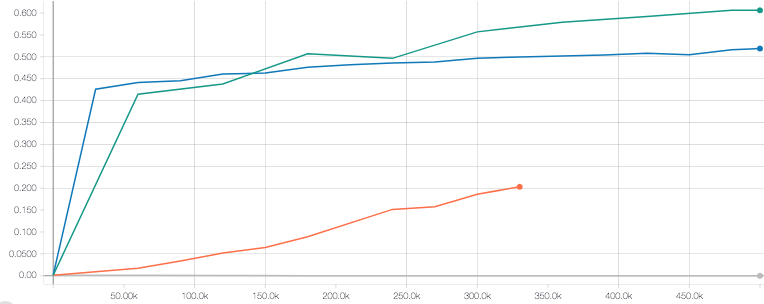
\includegraphics[width=\linewidth]{figures/multiobj/ex_vs_joint}
  \caption{Validation accuracy per time step. Green: multi-objective model (exclusive, rule-based) with interleaved input files. Blue: only exclusive objective. Orange: multi-objective model (exclusive, rule-based) loaded from the same training file (unstable). Shuffle queue: 15K.}
  \label{ex_vs_joint}
\end{figure}
\begin{figure}
  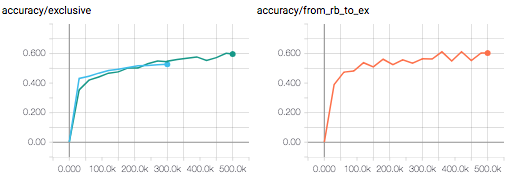
\includegraphics[width=\linewidth]{figures/multiobj/ex_vs_exclusivised}
  \caption{Validation accuracy per time step. Left green: exclusive objective in multi-objective training. Left blue: exclusive objective. Right orange: exclusivised objective. Shuffle queue: 100K.}
  \label{ex_vs_exclusivised}
\end{figure}

To assess whether the low accuracy of 60\% is caused by a genuine problem with learning or an ambiguous validation set, a confusion matrix was computed on the validation set.
Considering there were ~1000 categories, the heat map of the confusion matrix was too dense to reveal useful patterns.
Instead, a histogram of the number of categories that have a given misclassification rate was computed (figure \ref{misclassification_rates}); note that this was computed from both sides of the diagonal of the confusion matrix, therefore a misclassification is counted twice.
Top 20 categories with the highest misclassification rates are shown in figure \ref{misclassified_top}.
The categories with many misclassifications tend to be very general ones; for example, Clothing, Men's Clothing and Casual Shoes are certainly not exclusive, and the client company is advised to find ways of expressing these as exclusive categories.
For some (e.g. ``Knee Length'', ``Mini'', ``Tall''), visual information could be useful which in this round was not used.
The large number of categories that have a single or a handful of misclassifications is most likely caused by a learning problem such as insufficient labels or suboptimal training.

\begin{figure}
\centering
\begin{minipage}{.48\textwidth}
  \centering
  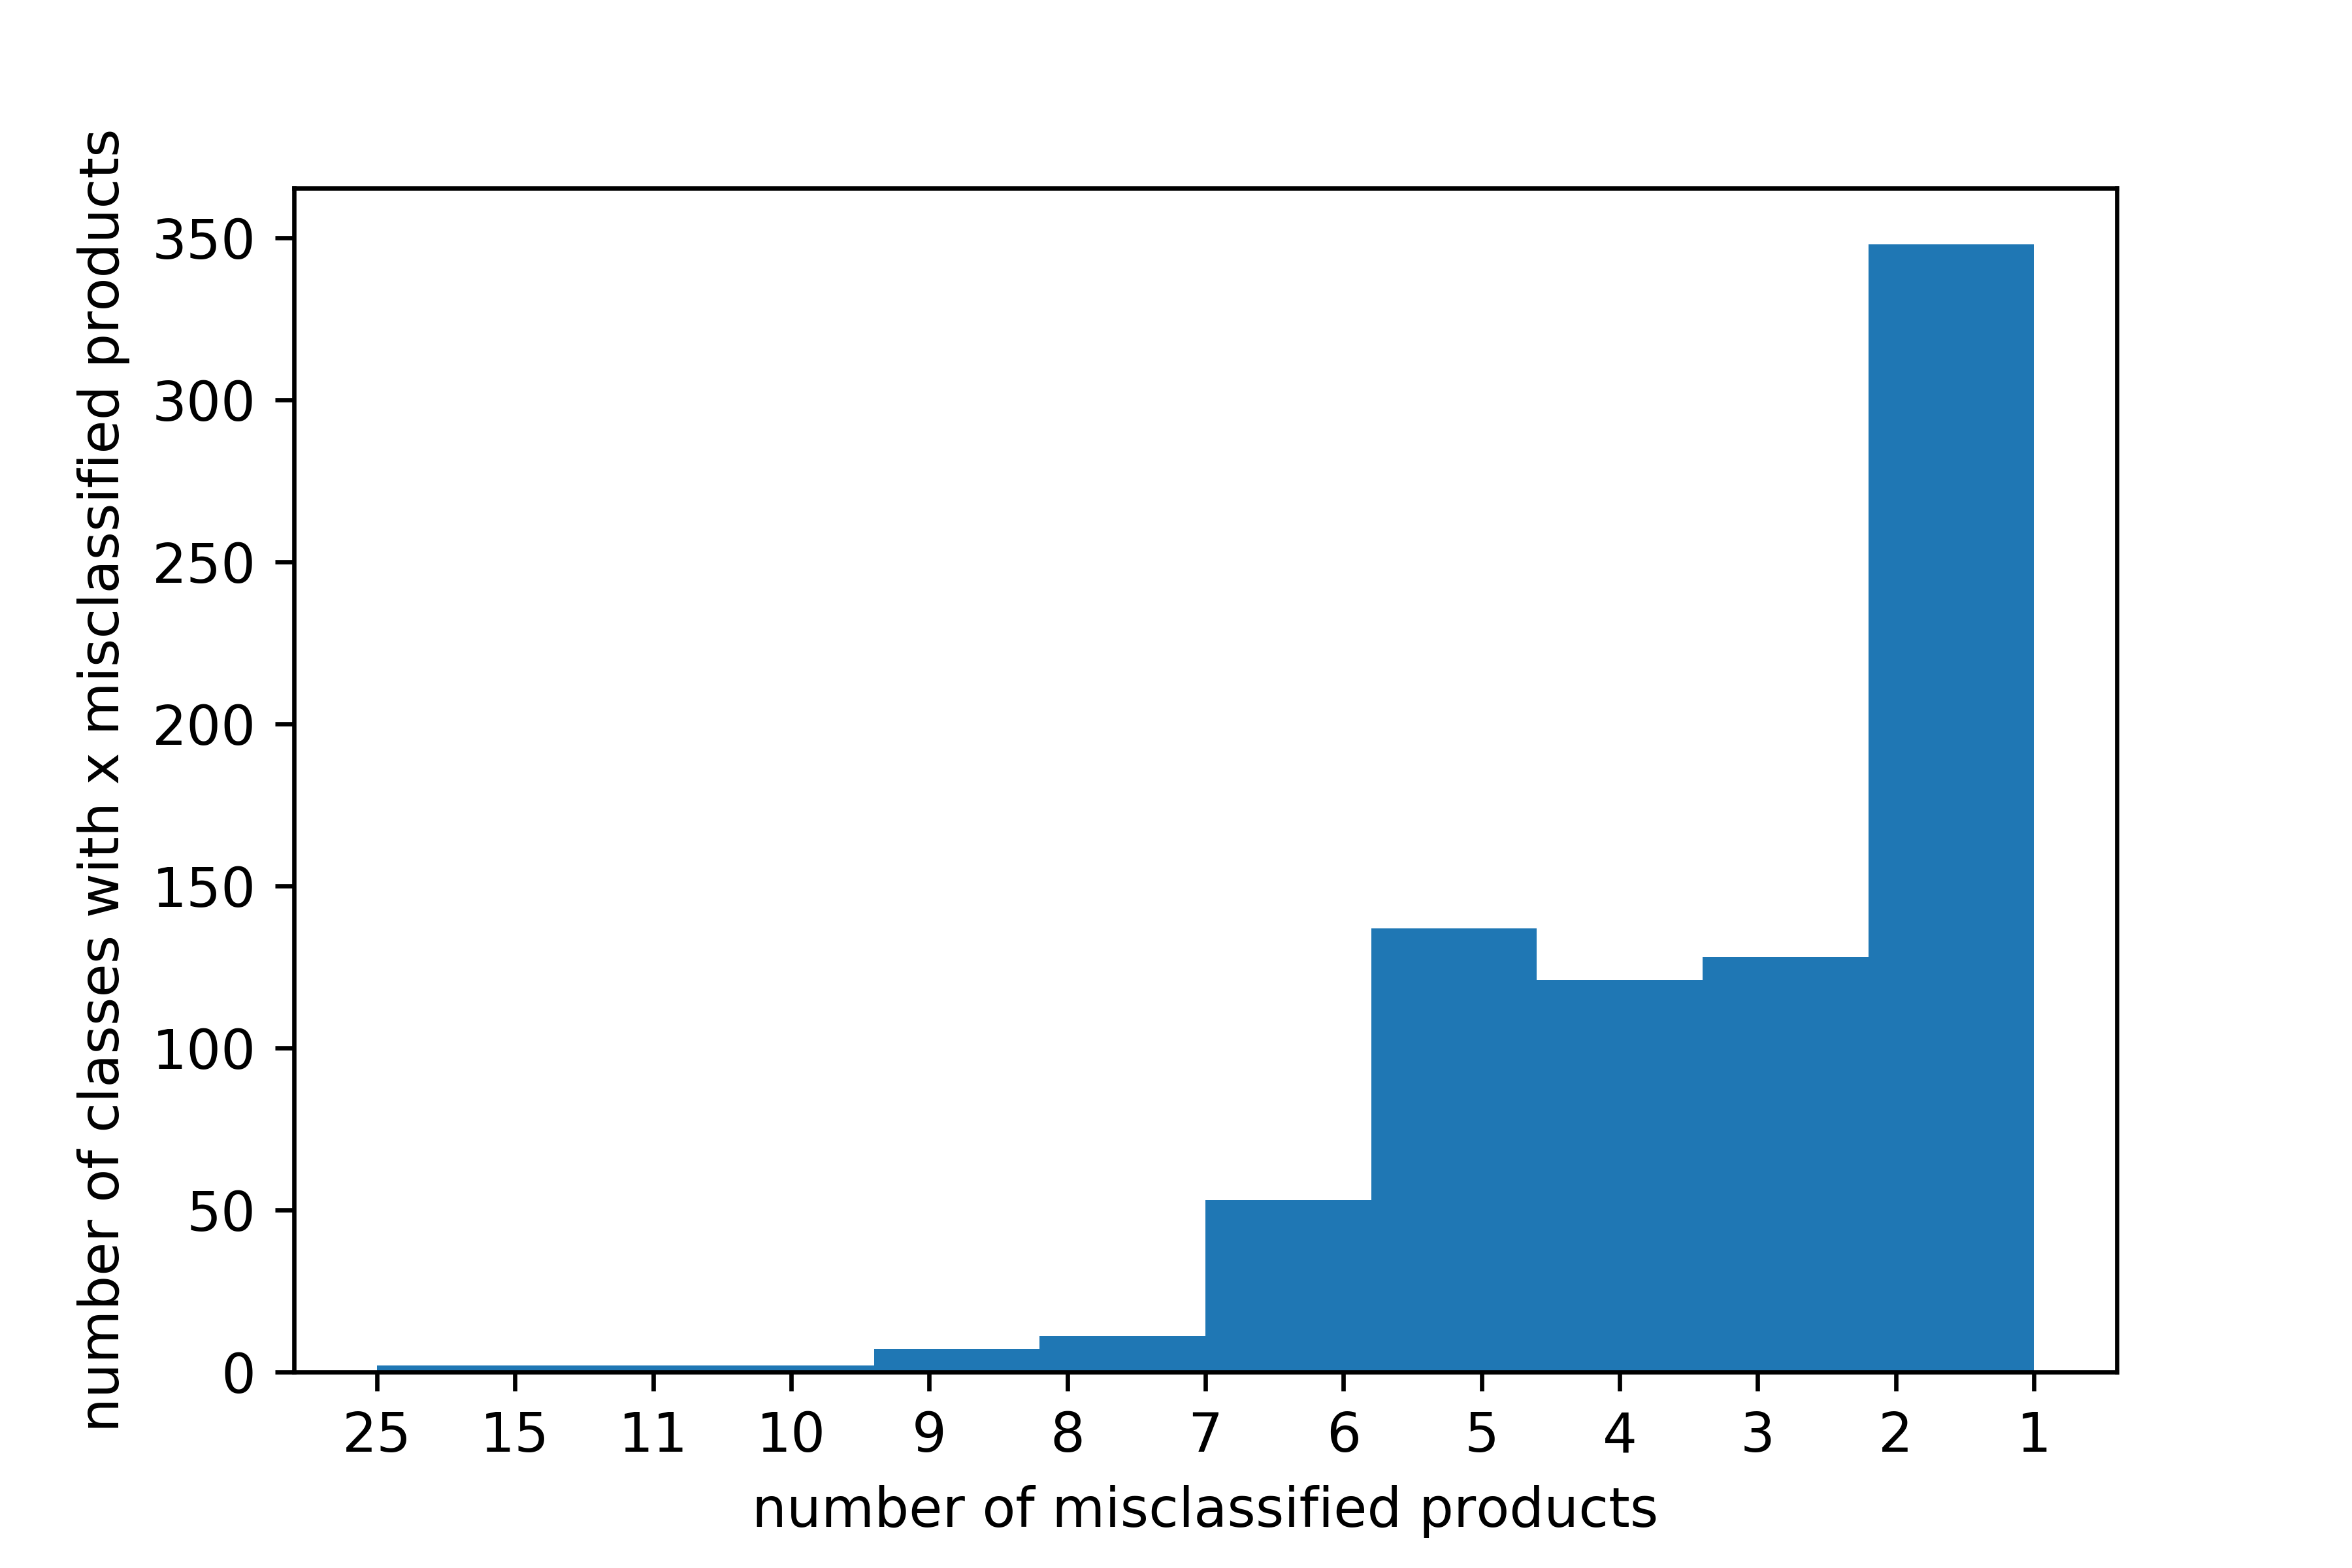
\includegraphics[width=\linewidth]{figures/multiobj/misclassification_rates}
  \caption{Number of misclassified products in validation set.}
  \label{misclassification_rates}
\end{minipage}%
\begin{minipage}{.48\textwidth}
  \centering
  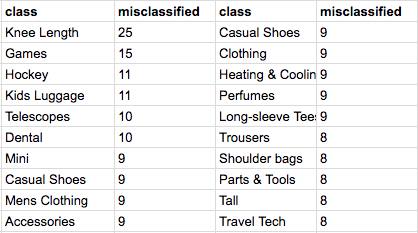
\includegraphics[width=\linewidth]{figures/multiobj/misclassified_top}
  \caption{Worst performers in validation set.}
  \label{misclassified_top}
\end{minipage}
\end{figure}


\section{Hyperparameter Selection \& Tuning}
\label{tuning}

Hyperparameters were chosen based on gut feeling and Bayesian optimisation.
The former was used to come up with reasonable ranges for hyperparameters; automatic tuning was done on the GCP ML Engine, where one just needs to specify the ranges of hyperparameters, their type (categorical, integer, reverse log scale), and how many models are trained in these hyperparameter ranges.
The ML Engine tuning mechanism uses Bayesian optimisation to come up with candidate hyperparameter values, which is described in section \ref{bayesian_opt} and by GCP engineers\footnote{https://cloud.google.com/blog/big-data/2017/08/hyperparameter-tuning-in-cloud-machine-learning-engine-using-bayesian-optimization}.
The hyperparameter ranges used and the results that each of the three tuning rounds found is shown in table \ref{tuning_rounds}.
In all cases 60 models were trained, with maximum 4 models trained in parallel, with early stopping.

The \textit{L2 scale} parameter is the weighting factor on the L2 regularisation term that is applied across the weights of the linear and deep models.
\textit{Linear learning rate} is the learning rate of the Adam optimiser for the linear part of Wide \& Deep, or the weights of the linear model; the other parameters of the optimiser were left as defaults (in TensorFlow and the original paper \cite{adam}); similarly for \textit{deep learning rate}.
Dropout corresponds to the likelihood of dropping out a hidden unit during training; \textit{layers} corresponds to the number of hidden layers, and \textit{hidden units} corresponds to the number of units in those hidden layers; \textit{activation} corresponds to the activation function used in the hidden layers; the four hyperparameters are only applicable to the deep and Wide \& Deep models.

Table \ref{tuning_rounds} shows the the tuning rounds in different colours, as well as the PR AUC achieved by each.
In the \textit{Wide \& Deep} case, tuning was performed over \textasciitilde800k data points on the rule-based objective, with each model trained up to 6 epochs (e.g. 125k time steps with a batch size of 64).
In the \textit{Deep (rb title)} case, a random sample of 10\% of the full 1.2M dataset was used to train on the rule-based objective for up to 50k time steps; the model used was deep\_title\_emb\_avg, which showed good results compared to the small selection of models that was manually tried.
In the \textit{Deep (exclusivised)} case, the deep\_noimg\_emb model was trained on the full 1.2M dataset on the \textit{exclusivised} objective (described in section \ref{multiobj}) for up to 300k time steps.
In the {Wide \& Deep} and \textit{Deep (rb title)} cases, models with a higher PR AUC score were preferred while in \textit{Deep (exclusivised)} accuracy was used to choose between hyperparameter performance.

It is clear that the hyperparameters found by the \textit{Deep (exclusivised)} round were not optimal, therefore the ones used in the \textit{Deep (rb all)} was used in most experiments described in section \ref{model_comb}.

\begin{figure}
  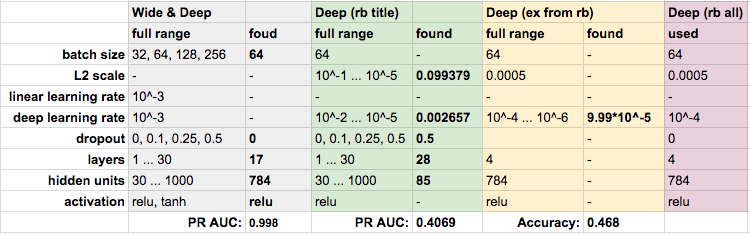
\includegraphics[width=\linewidth]{figures/tuning_rounds}
  \caption{Hyperparameter ranges and the values found during automatic tuning. A single value in the ``full range'' column means the value was fixed.}
  \label{tuning_rounds}
\end{figure}

\section{Active Learning}
\label{exp_al}

A limited experiment with active labelling was conducted.
After obtaining a small set of exclusive labels (as described in section \ref{labex}), the model noimg\_emb model was trained in a multi-objective setting, and the entropy of the exclusive objective was used to sample products to label.
In both cases, products were sampled 1-by-1 based on the entropy score (deterministically, highest entropy first).

Ideally we would have also tried disagreement sampling, but this would have involved loading predictions from different models across a large number of large files, which is not only slow but can easily introduce bugs related to misaligned predictions (i.e. products are in a different order across the predictions of different models). To store probabilities for 1000 classes across 4M products as 32bit floats, one needs 16GB; multiply that with the number of models you need to compare uncertainty between.

% Active labelling would be conducted in rounds.
% At each round, an equal number of products were labelled using random sampling and uncertainty sampling.
% After each round, three models were trained in a multi-objective manner.
% The rule-based objective is common to all three, but the number of exclusive labels is different in each: one is limited to randomly sampled labels, one is limited to uncertainty-sampled products, and one uses both.
% In all three cases the labels obtained in round 1 using text-based search were included.
% In this setting it should be possible to determine whether uncertainty sampling helps us increase validation accuracy faster than random sampling.

\subsection{Results}


The products returned by this method were in some sense what one might expect - at times returning products that were tricky to label or did not yet have a category - but the products were very similar to one another. As there is little value in herefore this labelling round was aborted.

\chapter{Discussion}
\label{disc}

In this section we analyse the experiments that were described in the previous section.

\section{Visual Similarity}

Although this assessment is subjective, the results from the approximate nearest neighbour were strikingly good; this is the opinion of many people at the client company that saw a demo of it.
The model did not require fine-tuning, contrary to the initial hypothesis.
The biggest challenge here is to find a way to evaluate visual similarity performance; although there are various algorithms for tweaking similarity and evaluating it on a test set, creating such a dataset would have been prohibitively expensive.
Given that vanilla pre-trained CNNs produce good embeddings for visual similarity, it is sensible to focus one's efforts on the scalability and productionalisation aspect of this problem.
Still, two relatively easy directions could yet be explored: the model architecture and the layer from which embeddings are extracted.
Our model of choice was Inception V3, which had a good accuracy to memory footprint ratio - with respect to the original ImageNet challenge.
However it has been shown that models that are well tuned for a given classification task are not necessarily the best feature extractors; in fact, ResNets are currently the best at this \cite{img_feature_extract}.
The other decision of of using the penultimate layer of the CNN as a feature extractor is also a common one.
Often the transfer learning task is classification, for which the higher-level fully-connected layers would provide good high-level semantic features.
In our case, extracting features from the first fully-connected layer or even from the raw convolutional feature maps at a lower layer might have given us similarity that is highly sensitive to certain visual patterns and shapes - which could be deployed to certain categories where such sensitivity is required.

As already discussed, the tokenised versions of feature vectors had less spectacular results.
While appealing as a way to combine visual and textual similarity, there is not theoretical justification for this approach.
Note that the original paper \cite{vec_fulltext} extracted dense features from text, and only hypothetically proposed this approach to be applied on images.
Perhaps the inherent discrete nature of language (sentences, words, topics as opposed to a continuous 2D space)  makes it more amenable to such tokenisation.

\section{Individual Models \& Hyperparameters}

Choosing a relatively complex model such as Wide \& Deep as a baseline model can be criticised: a baseline should be simple and interpretable.
One of the justifications was the ability to turn some part of the model off, as removing all deep input columns would have resulted in a linear model and vice versa\footnote{Implementing separate model types (deep, linear, wide \& deep) turned out to be simpler.}.
The other intuition was drawn from models with skip connections such as ResNets \cite{resnet} and DenseNets \cite{densenet}.
The assumption was that linear models are relatively good at predicting the output, as the relevant word tokens would be present in the textual fields of many products; for a deep model to use this raw knowledge, it would need to learn an identity function from the input of the layer to the output, which can be a hard problem with some activation functions.
Therefore, a linear layer with the same input as the deep layer could be justified to simplify learning for such simple cases, though not necessarily as the first ``baseline''.
Overall Wide \& Deep performed very well, though it is hard to compare its PR AUC to the other models, which were trained and evaluated on twice the amount of data.
When its performance degraded once it was trained on a new dataset (that most likely had mixed up image embeddings of some products), its drawback became apparent: we had no clue which of the input features were most responsible for good or bad performance.

Training a large selection of deep and shallow models was a good way to get a sense of the capabilities of these models.
The performance of linear models was lower than expected, but this is probably not a fair comparison, as the models were trained on the same sets of hyperparameters that were at least in part chosen to be suitable for deep models.
In general the tools used (TensorFlow, Adam optimiser) may not be optimal for learning linear models, but considering the large difference of PR AUC between the two, there seem to be benefits to using deeper models.
Contrary to our hypothesis, deep models with 1-hot / k-hot inputs did outperform shallow ones, but the difference in performance decreased when the models received a bigger selection of input features.
This implies that deep models are indeed generalising better from a small set of inputs; for example, the deep model that received averaged word embeddings of the title continued to improve even at epoch 6, and received a remarkably better PR AUC score (0.93) than its linear counterpart (0.42, or 0.53 for linear with k-hot inputs).

The biggest problem in interpreting the PR AUC scores of the rule-based objective is that its labels were generated using a relatively simple automatic procedure which only considers text as its input.
Therefore a high PR AUC score shows us only how well the model was able to reproduce the behaviour of the rule-based system, but we are after good generalisation and consistent multi-objective performance.
Therefore good results from title-only models should be taken with a grain of salt.
We consider the classification problem to be a quite easy optimisation problem, however the power of more complex models might be better served when we are adding more training objectives (e.g. colour, style, conversion of products).

Some patterns emerge from training this selection of models.
For linear models, 1-hot and k-hot encoding always outperforms embedding inputs, which was contrary to our hypothesis.
Deep models pre-trained on other objectives are quite consistent in their generalisation, producing strikingly similar PR AUC and recall scores whether it takes the title, description or image as input.
Examining the true/false positives/negatives of individual classes reveals that these models are relatively good at predicting certain classes, yet fail to differentiate between more specific ones.

It would be interesting to compare the performance of these models with random forests and 1D CNNs; fine-tuning of pre-trained models would also be an interesting comparison, as would models trained on character n-gram representations or TF-IDF-weighted embeddings.
Our embedding models could further be improved by not limiting the number of unique tokens so aggressively; as embedding based models have shown to perform better than 1-hot encoding in deep models, we could expand the vocabulary sizes without increasing input dimensionality.

Hyperparameter tuning using Bayesian optimisation was not as successful as expected.
In the first round where the Wide \& Deep model was tuned, the final metric value was only marginally higher than PR AUC of manually chosen hyperparameters, yet the model complexity was far greater.
A simpler model with comparable accuracy is more likely to generalise better, therefore most of the following deep models used 4 layers.
In the second tuning round, the model failed to learn in any instance; this is probably because the large range supplied for the ``L2 scale'' parameter.
An examination of the individual models that were trained during tuning showed that L2 decay overpowered the training loss and resulted in a very strict model that nearly always predicted the negative class.
The rate weight decay scaling parameter was kept fixed at 0.0005 for future runs based on analogous values used in literature; there is also some evidence that one should specify a custom scheme of weighting the L2 loss with adaptive optimisers such as Adam \cite{fix_adam}.

Given that we were training models with high capacity, it would also be useful to know the variance of the outcome if the model is trained several times by doing k-fold cross-validation.
Due to the large dataset size and time limitation this was not tried formally, however these models were trained across dozens of different data pre-processing runs during which the train/validation split was different.
There was not much variability within even the high-capacity models, which often converged at a high AUC PR score.

\section{Multi-Objective Training}

Even though the rule-based objective gave good PR AUC scores, the model was not deployable as is, since it severely under-predicted all nontrivial categories.
As one might expect, training for multiple objectives has a higher variance in the gradients.
This was exacerbated by the limitations of the tf.data APIs, which did not enable to efficiently alternate between the training objectives precisely.
Probably the variability could be reduced if each batch had a consistent number of products from each objective.
For more thorough experimentation, one should probably fall back to manually feeding data batch-by-batch, as was the standard in earlier versions of TensorFlow.

Although Adam was a versatile optimiser across the different deep and shallow architectures for the rule-based objective, updates to the parameters of each top layer becomes less frequent in the multi-objective case.
As Adam learns to update less frequently updated variables more heavily, this is probably the cause of a wide range of issues described in section \ref{multiobj}.
Note that it is not formally confirmed that the peculiarities are caused by adaptive learning rates.
Experimenting with a simpler optimiser and outputting per-step statistics about how many data points from each objective ended up in each bach would help further understand the shape of the loss functions.
For example, currently the best guess to the peculiar shape of the rule-based training loss (blue line in figure \ref{pretrain}) in a multi-objective training setting is that the large jumps are caused by a large batch of data points from the exclusive objective which has had few updates in a while; the medium-variance periods that follow such jumps (e.g. steps 40k - 80k) also contain data from that objective; the gradually decreasing plateaus (e.g. steps 80k - 120k and 170k - 200k) are periods where the model is trained only on the rule-based objective, which is considerably more stable.

It is satisfying that a multi-objective training scheme outperforms a method trained on just exclusive labels.
Though the exclusivised objective at times exceeds multi-objective training in terms of accuracy, the latter is preferred due to its stability and predictability; also, this scheme will be useful once we add additional training objectives.
The 60\% on the exclusive objective is not ideal.
This is achieved with roughly 6000 manual labels, which is far from the millions of labels deep neural networks usually require.
Probably the biggest gains will come from re-organising the category tree further so that there are no ambiguous classes, and that all the ambiguous cases (e.g. ``Leather Jackets'') are handled as a combination of an exclusive class (``Jacket'') and independent feature detector (``Material: leather'').
The remaining gains will come from active labelling, which should find the uncertain cases, or by manually adding labels to categories with a high error rate.
An orthogonal approach is to train using the Wasserstein loss, which would be better at handling ambiguous and noisy labels; in this case, we might use the Wasserstein distance between the predicted and actual labels as the evaluation metric as well, as accuracy would still paint a pessimistic picture when in reality it is acceptable to classify into a semantically nearby class.
Different training regimes could still be tried to stabilise multi-objective learning, such as gradient clipping, layer and batch normalisation.

A separate question is how to phase out the old rule-based system that the client company wishes to replace.
As the rule-based system would stop producing labels, any new products would be unlabelled according to it.
This would happen more often than one might think due to the way the data import process happens.
The most likely solution is to create an interface for mass-labelling of products: present the labeller pages with hundreds of products that are predicted to belong to a category, and have them confirm the page or pick out incorrect predictions.
This way we create a large number of high-quality labels with relatively little effort.

\section{Active Learning}

Preliminary results indicate that uncertainty sampling is effective at identifying products that might lack a category or sufficient labels in the training data, but it tends to sample products that are very much alike.
Therefore this strategy may not be very well suited for such a ``batch-active'' learning scenario as was presented.
A workaround might be a series of smaller training rounds.
Identifying unseen categories is a useful feature, though an analysis of validation error might produce similar results.

\chapter{Conclusion}
\label{sum}

In this work we covered a large breadth of topics.
Neural networks and deep models have many useful qualities: their performance continues to improve with additional training data, they can be successfully used for transfer and multi-task learning, and they can synthesise realistic samples of their own.
In general, deep models based on embedding inputs outperform ones with sparse inputs, while linear models do well with 1-hot encoded inputs.
Transfer learning is remarkably useful, as our experiments with visual similarity show, though models trained from scratch on raw product data is still superior for fine-grained affiliate product classification.
While this work did not experiment with ensembling of models, we did look at joint training of models that individually performed reasonably well, and as was expected found that a combination of all these inputs outperforms any subset.

A big part of the time spent on this project involved building the technical architecture.
This was a non-trivial task given the large number of technologies, distributed components and dataset sizes involved.
This could serve as a blueprint for many projects that are planning to deploy to the GCP cloud.

Our experiments with multi-objective training ultimately produced the expected results, and the performance increase could be hopefully improved with more analysis of the high gradient variance during training.
Even though a good number of models were trained to optimise hyperparameters using Bayesian optimisation, the bulk of these were still picked based on intuition.
At the very least, such tuning reveals that at least for this problem the models are not too sensitive to hyperparameters.

The results from active learning are not yet conclusive, though the tentative conclusion is that uncertainty sampling should not be used too early when the model is not yet close to an optimal solution, as it might sample very similar data points.
Our experiments are still in progress, though, and a later evaluation might conclude something more positive.

Overall, the choice of tools and approaches was reasonable.
There are clearly more straightforward ways to do product classification, yet the complications introduced by transfer, multi-objective and active learning will most likely pay off when predicting much more difficult aspects, such as whether a product would sell well for a given audience or not - which has immense potential to increase profitability.


\renewcommand\bibname{References}
\bibliographystyle{plain}
\bibliography{extras/_bibliography}

\clearpage
\pagestyle{empty}
% \renewcommand*{\chapterpagestyle}{empty}
\chapter*{Declaration}




\vspace*{2cm}
\noindent
I hereby certify that I have written this thesis independently and have only used the specified sources and resources indicated in the bibliography.

\vspace{2cm}

\noindent
London, UK, \today

\vspace{3cm}

\hspace*{7cm}%
\dotfill\\
\hspace*{8.5cm}%
\textit{Mattias Arro}
\addcontentsline{toc}{chapter}{Declaration}


\appendix
\addappheadtotoc
\chapter{Additional Background}

\section{Neural Models}

\subsection{1D Convolutional Neural Networks}
\label{1d_cnn_app}

A simple convolutional architecture for text classification is described in \cite{1dcnn}.
Pre-trained $k$-dimensional word vectors are concatenated to represent a sentence, and a filter is $w \in R^{hk}$ is applied to a window of $h$ words at each possible window of words in a sentence; this gives a single variable-length feature vector representing the sentence.
Several such filters are learned (each with potentially a different width $h$), and max-over-time pooling is applied to these feature maps; this gives a vector of the highest activations from each filter, which is then passed to a fully-connected softmax or sigmoid layer for final classification.

This simple architecture should be able to predict output classes reasonably.
Each filter can indicate the presence of a a sequence of $h$ words; max-pooling discards information about where exactly in the text it appeared, and ensures the output is of a fixed length.
The same filter $w$ is used across all possible word windows in the sentence, which can be seen as a form of parameter sharing (and as an infinitely strong prior over the parameters of the model \cite{dlb}), and enables processing variable-length sequences.
The relatively small number of shared parameters requires less training data than an equivalent fully-connected architecture.
Using pre-trained word embeddings further simplifies the task, as these already carry some information about the meaning or syntactic role of words.

More sophisticated architectures can be built using 1D CNNs, although not used in our experiments.
Most notably, several layers of convolutions and pooling can be stacked, where the following layer works on the feature maps output by the previous layer.
The model described above uses a stride and dilation of 1, but multi-layer architectures where the higher layers have use exponentially increasing dilation are able to expand the receptive field of the model, and as a result aggregate ``contextual information from multiple scales'' \cite{dilated}.
Dilated convolutions were beneficial for semantic segmentation of images with 2D CNNs; increased receptive field has also been benefitial in sequence-to-sequence NLP models \cite{dilated_decoder}.

\subsection{Recurrent Neural Networks}
\label{rnn_app}

Recurrent neural networks (RNNs) are a family of models for processing sequential data.
The sequence of inputs $x^{(1)} \dots x^{(t)}$ in our case are vectors of word embeddings, but there are other options for input representations (e.g. sequence of 1-hot encoded tokens, or vectors representing a multivariate time series at a given time step $t$).
Vanilla RNNs maintain a hidden state vector $h$ which contains some information about the sequence it has seen so far, and is calculated from the input at the current time step $t$, and the previous hidden state:

\begin{equation}
  h^{(t)} = f(h^{(t-1)},x^{(t)})
\end{equation}

Vanilla RNNs suffer from the vanishing and exploding gradient problem in long sequences and are notoriously difficult to train.
Probably the most widely used variant, the long short-term memory networks (LSTM) \cite{lstm} overcome this limitation by augmenting the network with a memory cell $c$; there is a learned gating mechanism that controls what part of (and the extent to which) the cell is forgotten, what gets persisted in the cell state, and what gets output at a given time step.
An intuitive overview of the gating mechanisms is given by \cite{colah} and \cite{vanishing} describes well how this helps mitigate vanishing gradients.
A simpler gating mechanism is offered by gated recurrent units (GRU) \cite{gru}, which has fewer parameters and works well on simpler tasks.

We are interested in using RNNs as text encoders, though they are often used for sequence to sequence modelling, or for predicting an output at each time step.
In the simplest case, the concatenation of the cell state $c$ and the hidden state $h$ at the last time step could be used as a representation of the sequence.

\section{Unsupervised and Semi-supervised Learning}
\label{unsup_appendix}

This section explores ways in which unsupervised and semi-supervised learning can learn good feature representations and improve label complexity.
Generic semi-supervised methods such as self-training are not considered, as one of our goals is to learn good representations, but also because these methods can reinforce poor predictions or do not make full use of all available unlabelled data.

Some generic methods can still improve the representations learned by our models when applied to models that learn deep embeddings in order to make predictions.
Entropy minimisation \cite{entropy_min} can be incorporated into models trained with SGD to encourage confident predictions of each class; this encourages the deep model to learn predictions that are strong predictors of some class and avoid producing features that produce mixed predictions.
More complex but very performant approach is Mean Teacher \cite{mean_teacher}. A student that gets a harder task (such as predicting from a noisy/adversarial example), and a teacher that gets an easier task (i.e. the teacher model is an ensemble, which is more accurate).
The student is trained on the prediction of the teacher; the teacher's parameters are an exponential moving average of the student's, updated after each minibatch.
The teacher's predictions are higher-quality than the student's (and can be applied on unlabelled data), while the student tries to continuously learn to learn a predictor that is robust to noisy and adversarial examples.

\subsection{Autoencoders \& Variational Autoencoders}

Deep autoencoders (AEs) can be used to learn low-dimensional representations of inputs.
Many variants exist,  but  the general pattern is to have an ``hourglass-structured'' neural network where the first half of the model shrinks the input, and the second half of the network reconstructs it.
Activations in the middle layer correspond to a dense embedding of the sample;  the shrinking layers need to  throw away some of the detail in the input, yet persists enough for the expanding layers to be able to reconstruct the original input with some fidelity.
The embedding contains information that is mostly unique to the data point, while the parameters of the encoding and decoding layers ensure that the reconstructed input is realistic.
It is common to add noise (Gaussian, dropout) to the input or the intermediate layers to increase resilience to noisy inputs and to prevent the autoencoder simply memorising each data point.

If the bottleneck layer is unconstrained, it will use a wide range of values to represent different inputs.
We would like embedding for similar inputs to also be similar, which is not always the case for ordinary autoencoders.
Variational autoencoders (VAEs) impose a prior distribution on the values of the embedding $z$, often a multivariate Gaussian distribution with a diagonal covariance matrix, and the model is regularised during training to respect this prior.
The model is optimised to minimise the reconstruction loss and KL divergence between the model's distribution of and the prior on it, which can be computed just from $\mu(z)$ and $\sigma(z)$ if the prior is a isotropic standard normal.
Enforcing the prior also means that the embeddings $z$ will occupy a smooth, contiguous space, which allows us to draw samples from the prior $\epsilon \sim \mathcal{N}(0, 1)\,$ and use that as the input to the decoder - this gives us a generative model, which would not be possible with ordinary autoencoders.
The output of the VAE is also probabilistic: e.g. for images, the output for a pixel would be a Gaussian distribution, which is sampled the same way as the Gaussians for $z$.

The VAEs described here are probabilistic models parameterised by neural networks for approximating the true posterior $p(z|x)$, since the exact posterior is intractable.
In practice, VAEs add an extra loss term (KL divergence) to AEs, and additional step to determining the embedding $z$.
There are two separate neural network layers from the bottleneck layer of the AE:  one for determining $\mu(z)$ (the vector of means of the multivariate Gaussian), and one for determining $\sigma(z)$ (the vector of standard deviations of the multivariate gaussian).
Given $\mu(z)$ and $\sigma(z)$, we can sample the final item embedding $z \sim \mathcal{N}(\mu,\,\sigma^{2})\,$.
Note that sampling of $z$ is a discrete decision that would normally stop gradient from propagating past this step, but we can use the reparametrisation trick introduced by \cite{vae} that turns the discrete decision into a deterministic function of $z = \mu + \sigma\epsilon$, where $\epsilon \sim \mathcal{N}(0, 1)\,$ is a random auxiliary noise parameter.


\subsection{Conditional Variational Autoencoders}
\label{gans}
It is easier for linear models to learn from embeddings extracted with AEs, and embeddings from VAEs make the classes even easier to separate.
These are unsupervised methods that do not take advantage of labels in the training data.
In the semi-supervised approach introduced by \cite{semi_vae} there are two inference networks: a discriminative classifier that outputs a categorical distribution from the input $x$, and a class-conditional encoder that takes as input both $x$ and the 1-hot encoded categorical label $y$\footnote{Class-conditional encoder means that the encoder is aware of the class of the data point, i.e. the output distribution $z$ is conditioned on the class $y$ in addition to the original input $x$.}.
The model is trained on both labelled and unlabelled data.
For labelled examples, the $x$ and $y$ are given as input to the model, which embeds it in $z$ as described earlier, and reconstructs the original $x$.
The value of $y$ is unknown for unlabelled data points; therefore the model is run $|y|$ times, encoding and decoding the data point conditioned on each possible class $i$; loss from these runs is averaged, weighted by the discriminator's estimate of the sample belonging to class $i$.
This approach is acceptable for small numbers of classes, but is impractical for many multi-class problems.
A solution uses the reparametrisation trick mentioned above: rather than running the procedure once per class, we take a Gumbel-softmax \cite{gumbel} to get a discrete estimate of $y$ that is still differentiable.

Such class-conditional VAEs can be used in any situation where unlabelled data is abundant but labels are scarce.
The discriminator's loss is optimised as part of the VAE's loss function, which means adding more unlabelled data can improve the accuracy of the discriminator.
The approach was developed and tested on the MNIST dataset, which consists of 28x28 grayscale images - a very simple dataset by today's standards.
Some reports have emerged that fail to reproduce this success on more complex datasets such as CIFAR-10, being outperformed even by PCA \cite{vae_bad}.

One related approach is offered by \cite{towards}, where a class-conditional VAE is used to generate synthetic data for a discriminator network, which has reportedly a higher accuracy in semi-supervised setting than the approach described just above.
They use it for conditional text generation, but this approach of using the class-conditional VAE to synthesise training data to train a discriminator is applicable to any input modality.
In fact the general approach to ``dreaming up'' new training samples in the \textit{sleep phase} and training the classifier in the \textit{wake phase} was introduced already in \cite{wake_sleep}.
The current author has implemented this model and open sourced it\footnote{https://github.com/mattiasarro/seq2seq-cvae-tensorflow}.

\subsection{Generative Adversarial Networks}

Generative adversarial networks (GANs) are an interesting approach capable of synthesising realistic data, but also useful for learning good representations of data.
GANs have been most successful for image synthesis, but are in fact applicable to any kind of input data including text \cite{textgan} and even mixed data types such as e-commerce orders \cite{ecomgan}.
In the GAN setting, there are two networks: a generator that tries to produce realistic synthetic samples, and a discriminator whose goal is to distinguish between synthetic and actual samples.
% The networks are trained as a min-max optimisation problem where the generator is optimised to ``fool'' the discriminator by producing samples that appear to come from the true distribution, and the discriminator is optimised to  determine which samples are synthetic.
Given that the training is stable enough, both the generator's and the discriminator's performance improves with time, resulting in more realistic synthetic samples, as opposed to the relative blurry images produced by VAEs.
The discriminator needs to learn good representations of the input to  accurately distinguish which samples come from the true distribution, and which samples are synthetic; as with many CNNs for computer vision, these representations can be useful for other tasks as well.

It has been shown that  linear models  from the embeddings learned by the discriminator outperform other unsupervised feature learning techniques such as k-means \cite{dcgan}.
At the time of writing, variants of Wasserian GANs (WGANs) achieve the best performance by improving training stability and preventing the generator from generating samples from a limited number of modes; this is achieved by minimising the Wasserian distance between the generator's and real data distributions, as opposed to minimising the JS divergence as was common before.
A performant variant of WGAN is CT-GAN, which adds a regularisation term to enforce a Lipschitz continuity condition over the manifold of the real data \cite{ctgan}.


\end{document}
